\section{Shape Sensitivity of Flow over a Cylinder}
% ==================================================
For the second demonstration problem, the flow over a cylinder is modeled using the virtual boundary method using Equation \eqref{eq:C4_NSwithvirtualBoundaryIB} and the sensitivity of the flow field variables (velocity and pressure) with respect to the radius of the cylinder is calculated. For this problem the domain is defined as a rectangle with the cylinder located on the horizontal symmetry line as shown in Figure \ref{fig:C4_cylinderPhysicalDomain}.

\begin{figure}[H]
    \centering
    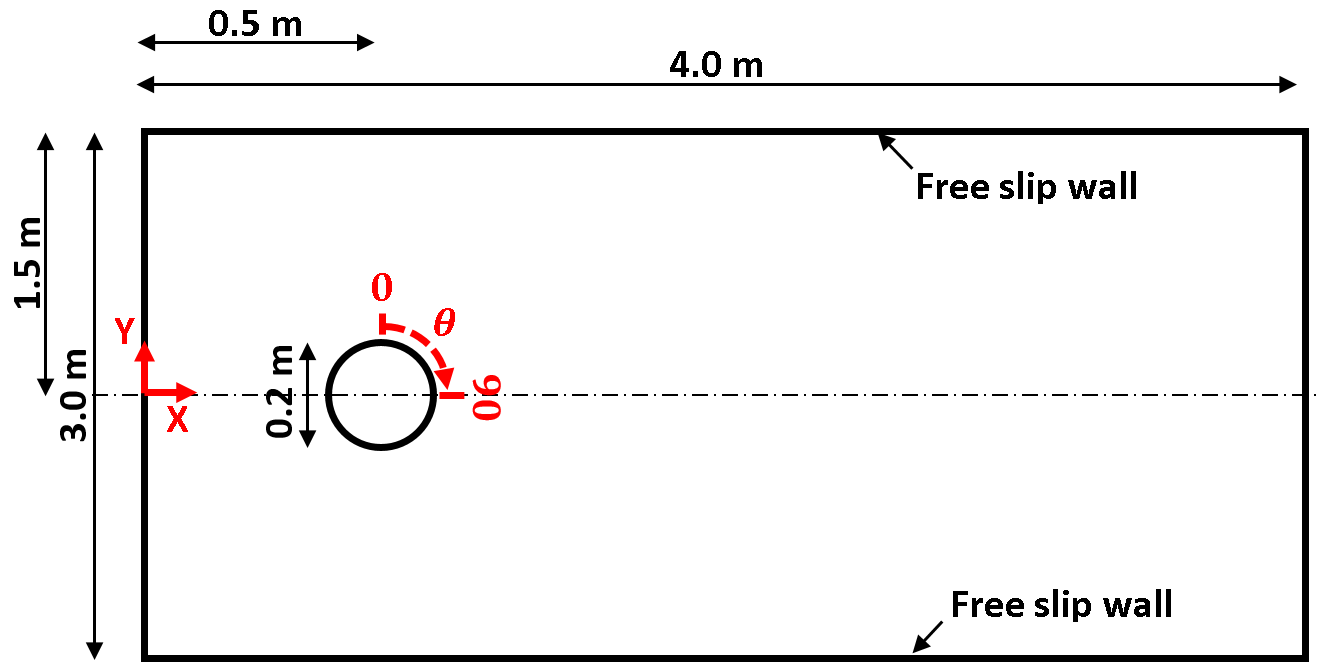
\includegraphics[width=12.00cm]{Chapter_4/figure/flow_over_cylinder/flow_over_cylinder.png}
    \caption{Physical domain with dimensions for flow over cylinder.}
    \label{fig:C4_cylinderPhysicalDomain}
\end{figure}

The boundary conditions are defined as the flow velocity at the inlet (left boundary) and the outflow (zero gradient) boundary condition at the outlet (right boundary). The top and bottom boundaries are modeled as free slip walls. The surface of the cylinder is modeled by the virtual boundary method. The cylinder is located at $(0.5, 0.0)$ and has the radius of $0.1 m$. Its surface is represented by using 100 Lagrangian nodes. The $\alpha$ and $\beta$ values for this analysis are selected as $-10^4$ and $-50$. These constants are problem dependent and are selected in such a way that the required velocity conditions are satisfied at the Lagrangian points. To ensure the stability of the numerical method, the CFL number is kept under one for all the following analysis. This is done by selected the appropriate time step for the chosen mesh size using Equation \eqref{eq:C4_CFLnumber}.

\begin{equation}\label{eq:C4_CFLnumber}
	\frac{u \Delta t}{\Delta x} + \frac{v \Delta t}{\Delta y} \leq 1.0
\end{equation}


The mesh convergence for this problem for Reynolds number of 100 is shown in Figure \ref{fig:C4_meshConvergenceForCylidnerRE100GE}.

\begin{figure}[H]
    \centering
    \subfigure[U-velocity on y = 0.]
    {
    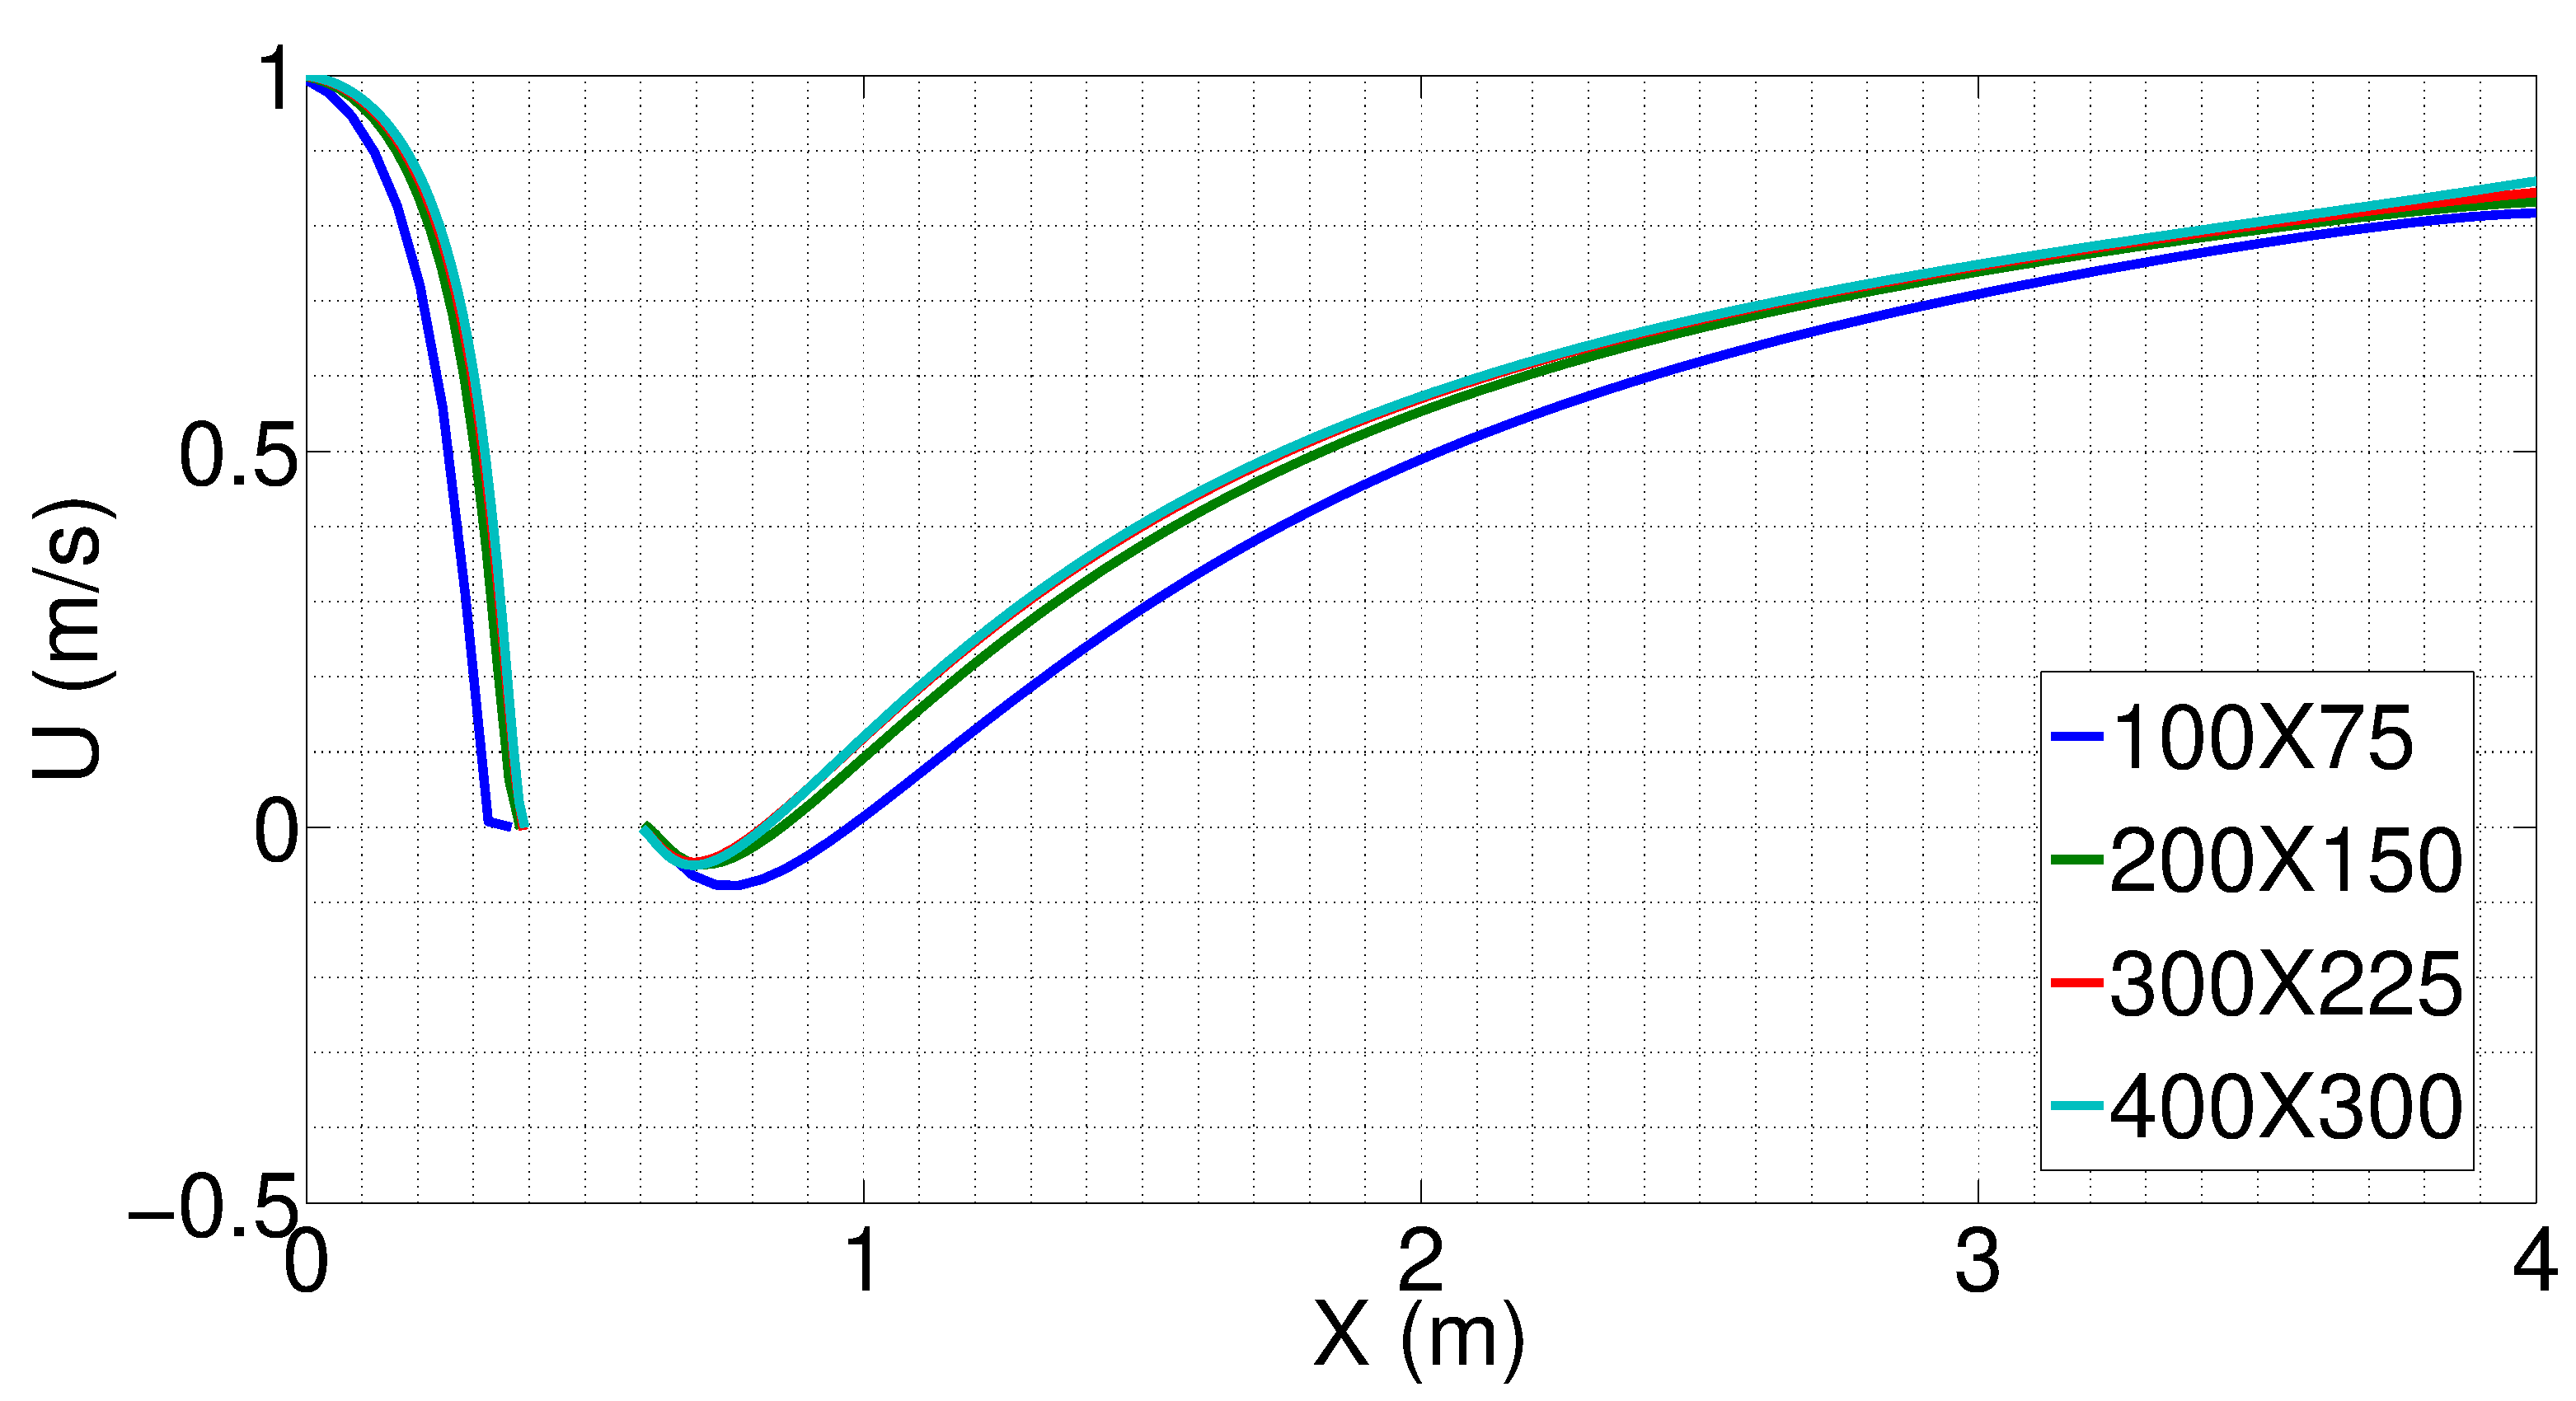
\includegraphics[width=7.0cm]{Chapter_4/figure/flow_over_cylinder/meshConvergence_RE100_U.eps}
    }
    \quad
    \subfigure[V-velocity on x = 0.5]
    {
    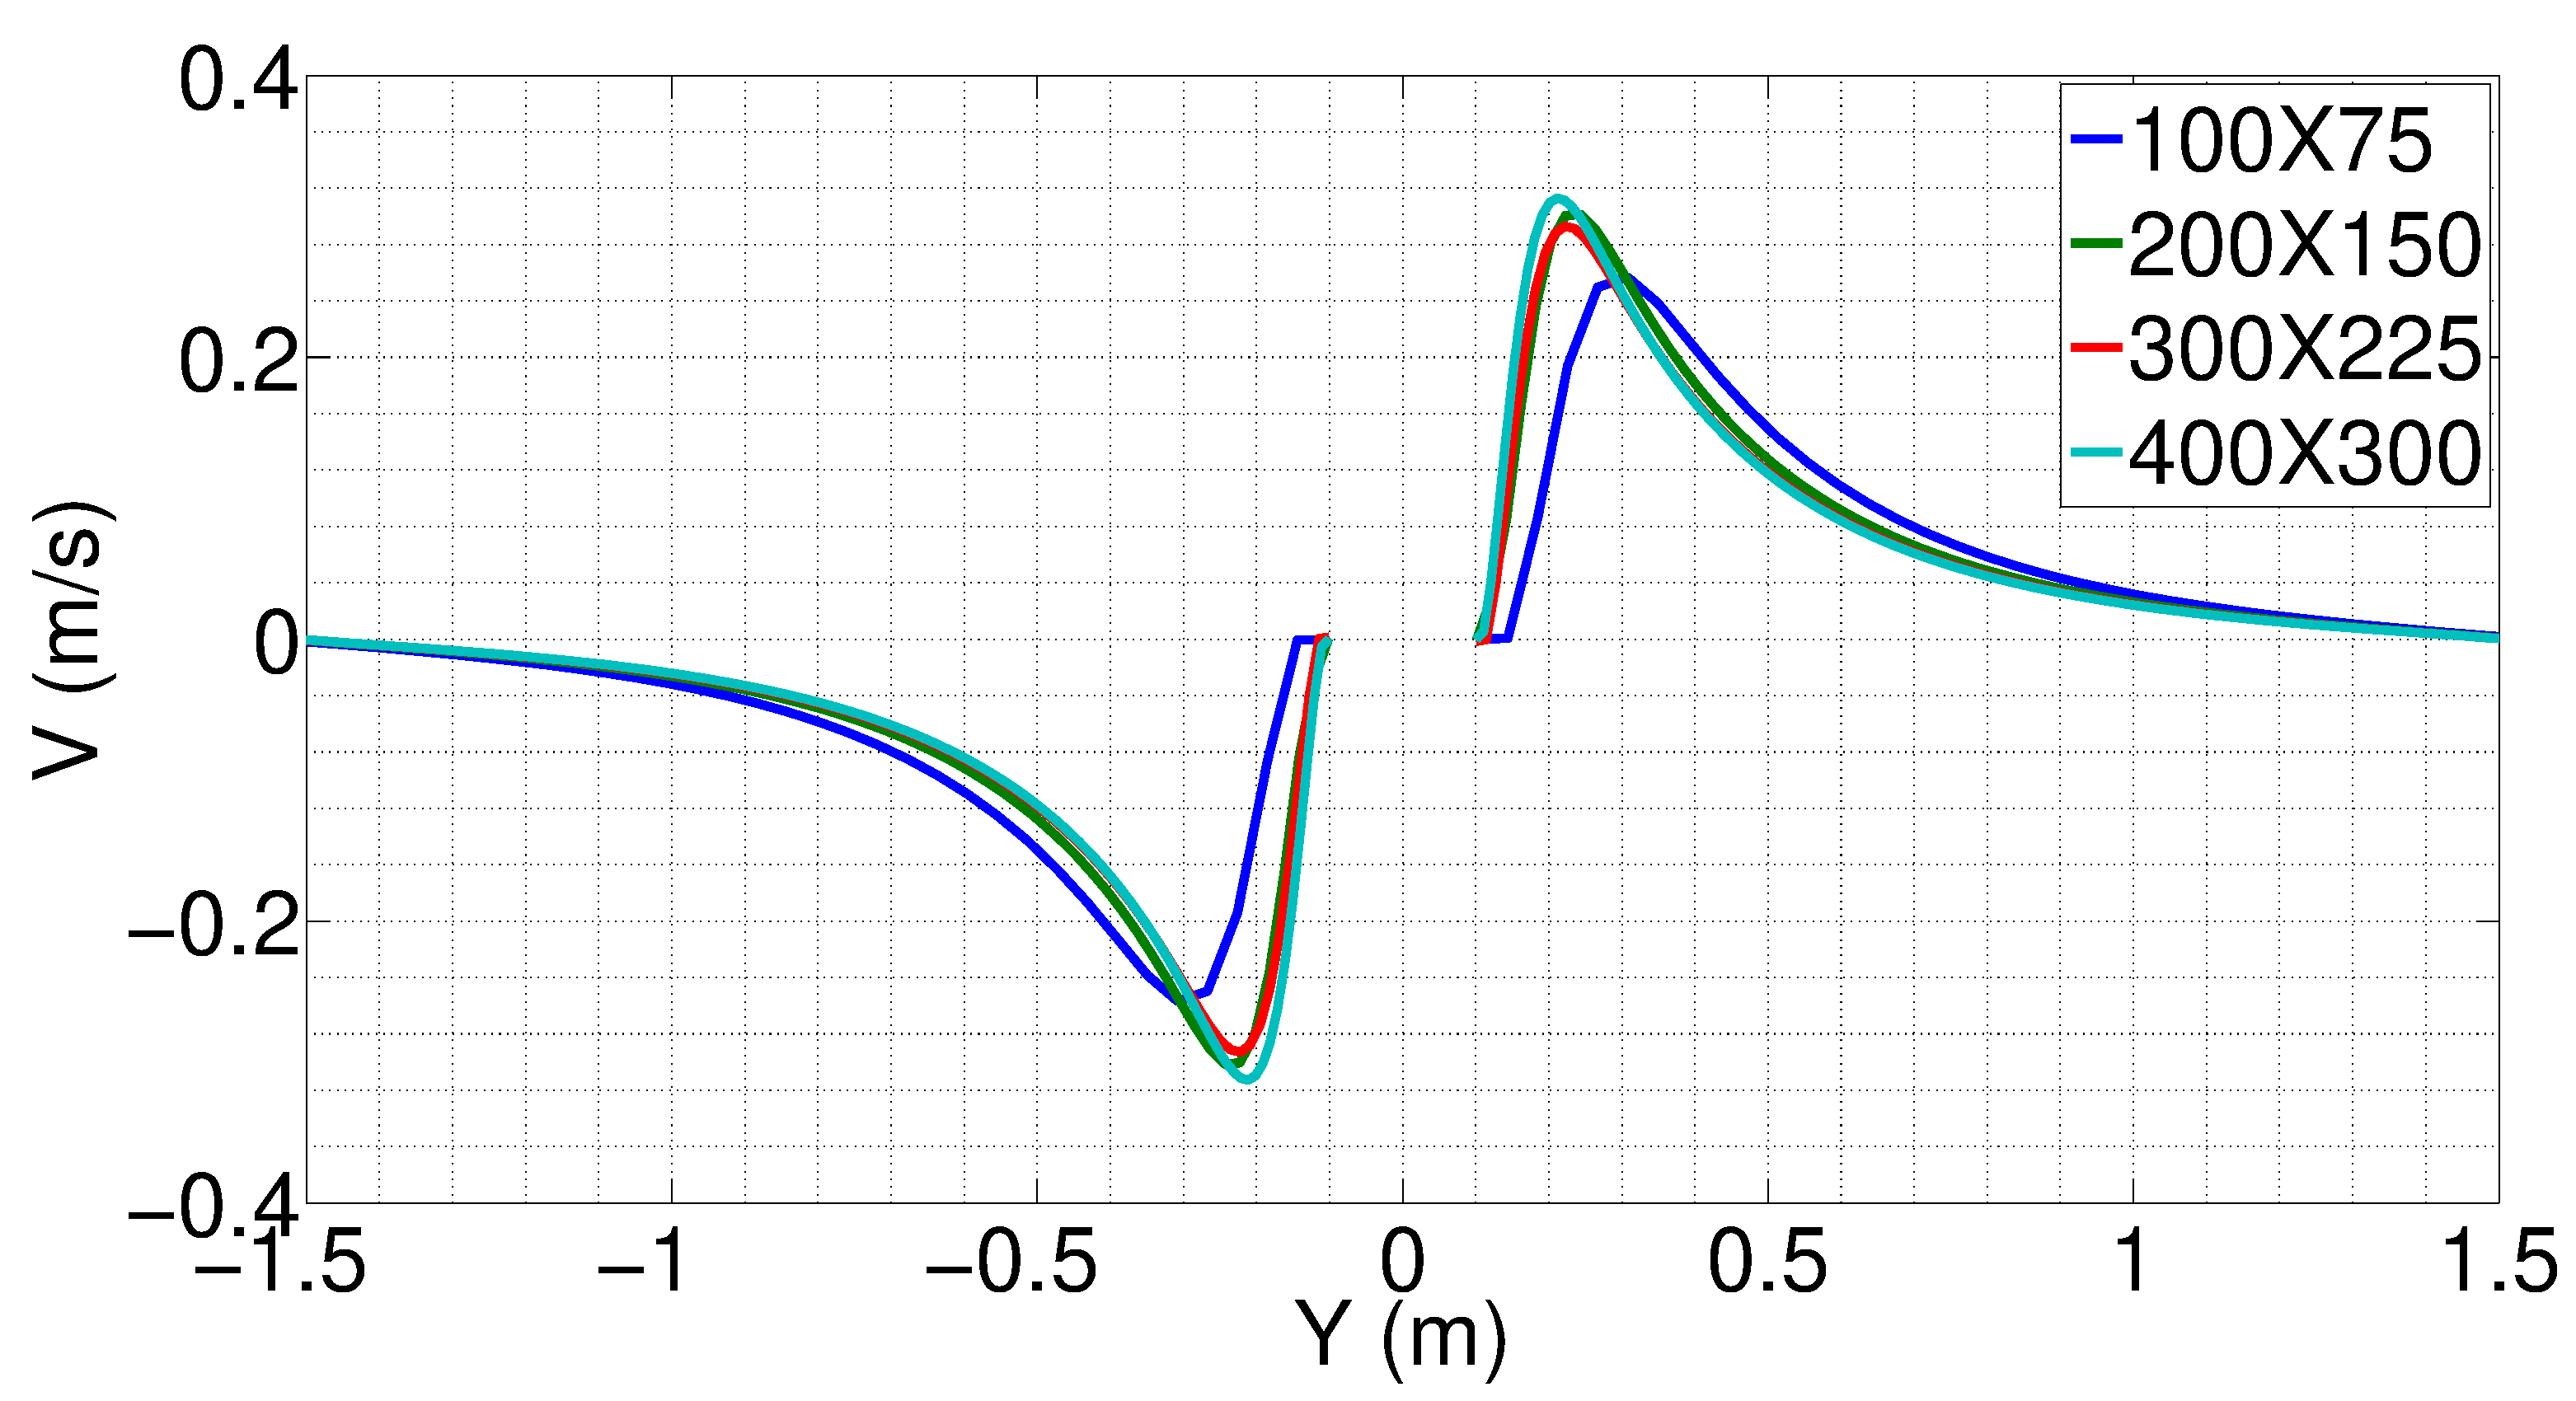
\includegraphics[width=7.0cm]{Chapter_4/figure/flow_over_cylinder/meshConvergence_RE100_V.eps}
    }
    \\
    \subfigure[Pressure on y = 0]
    {
    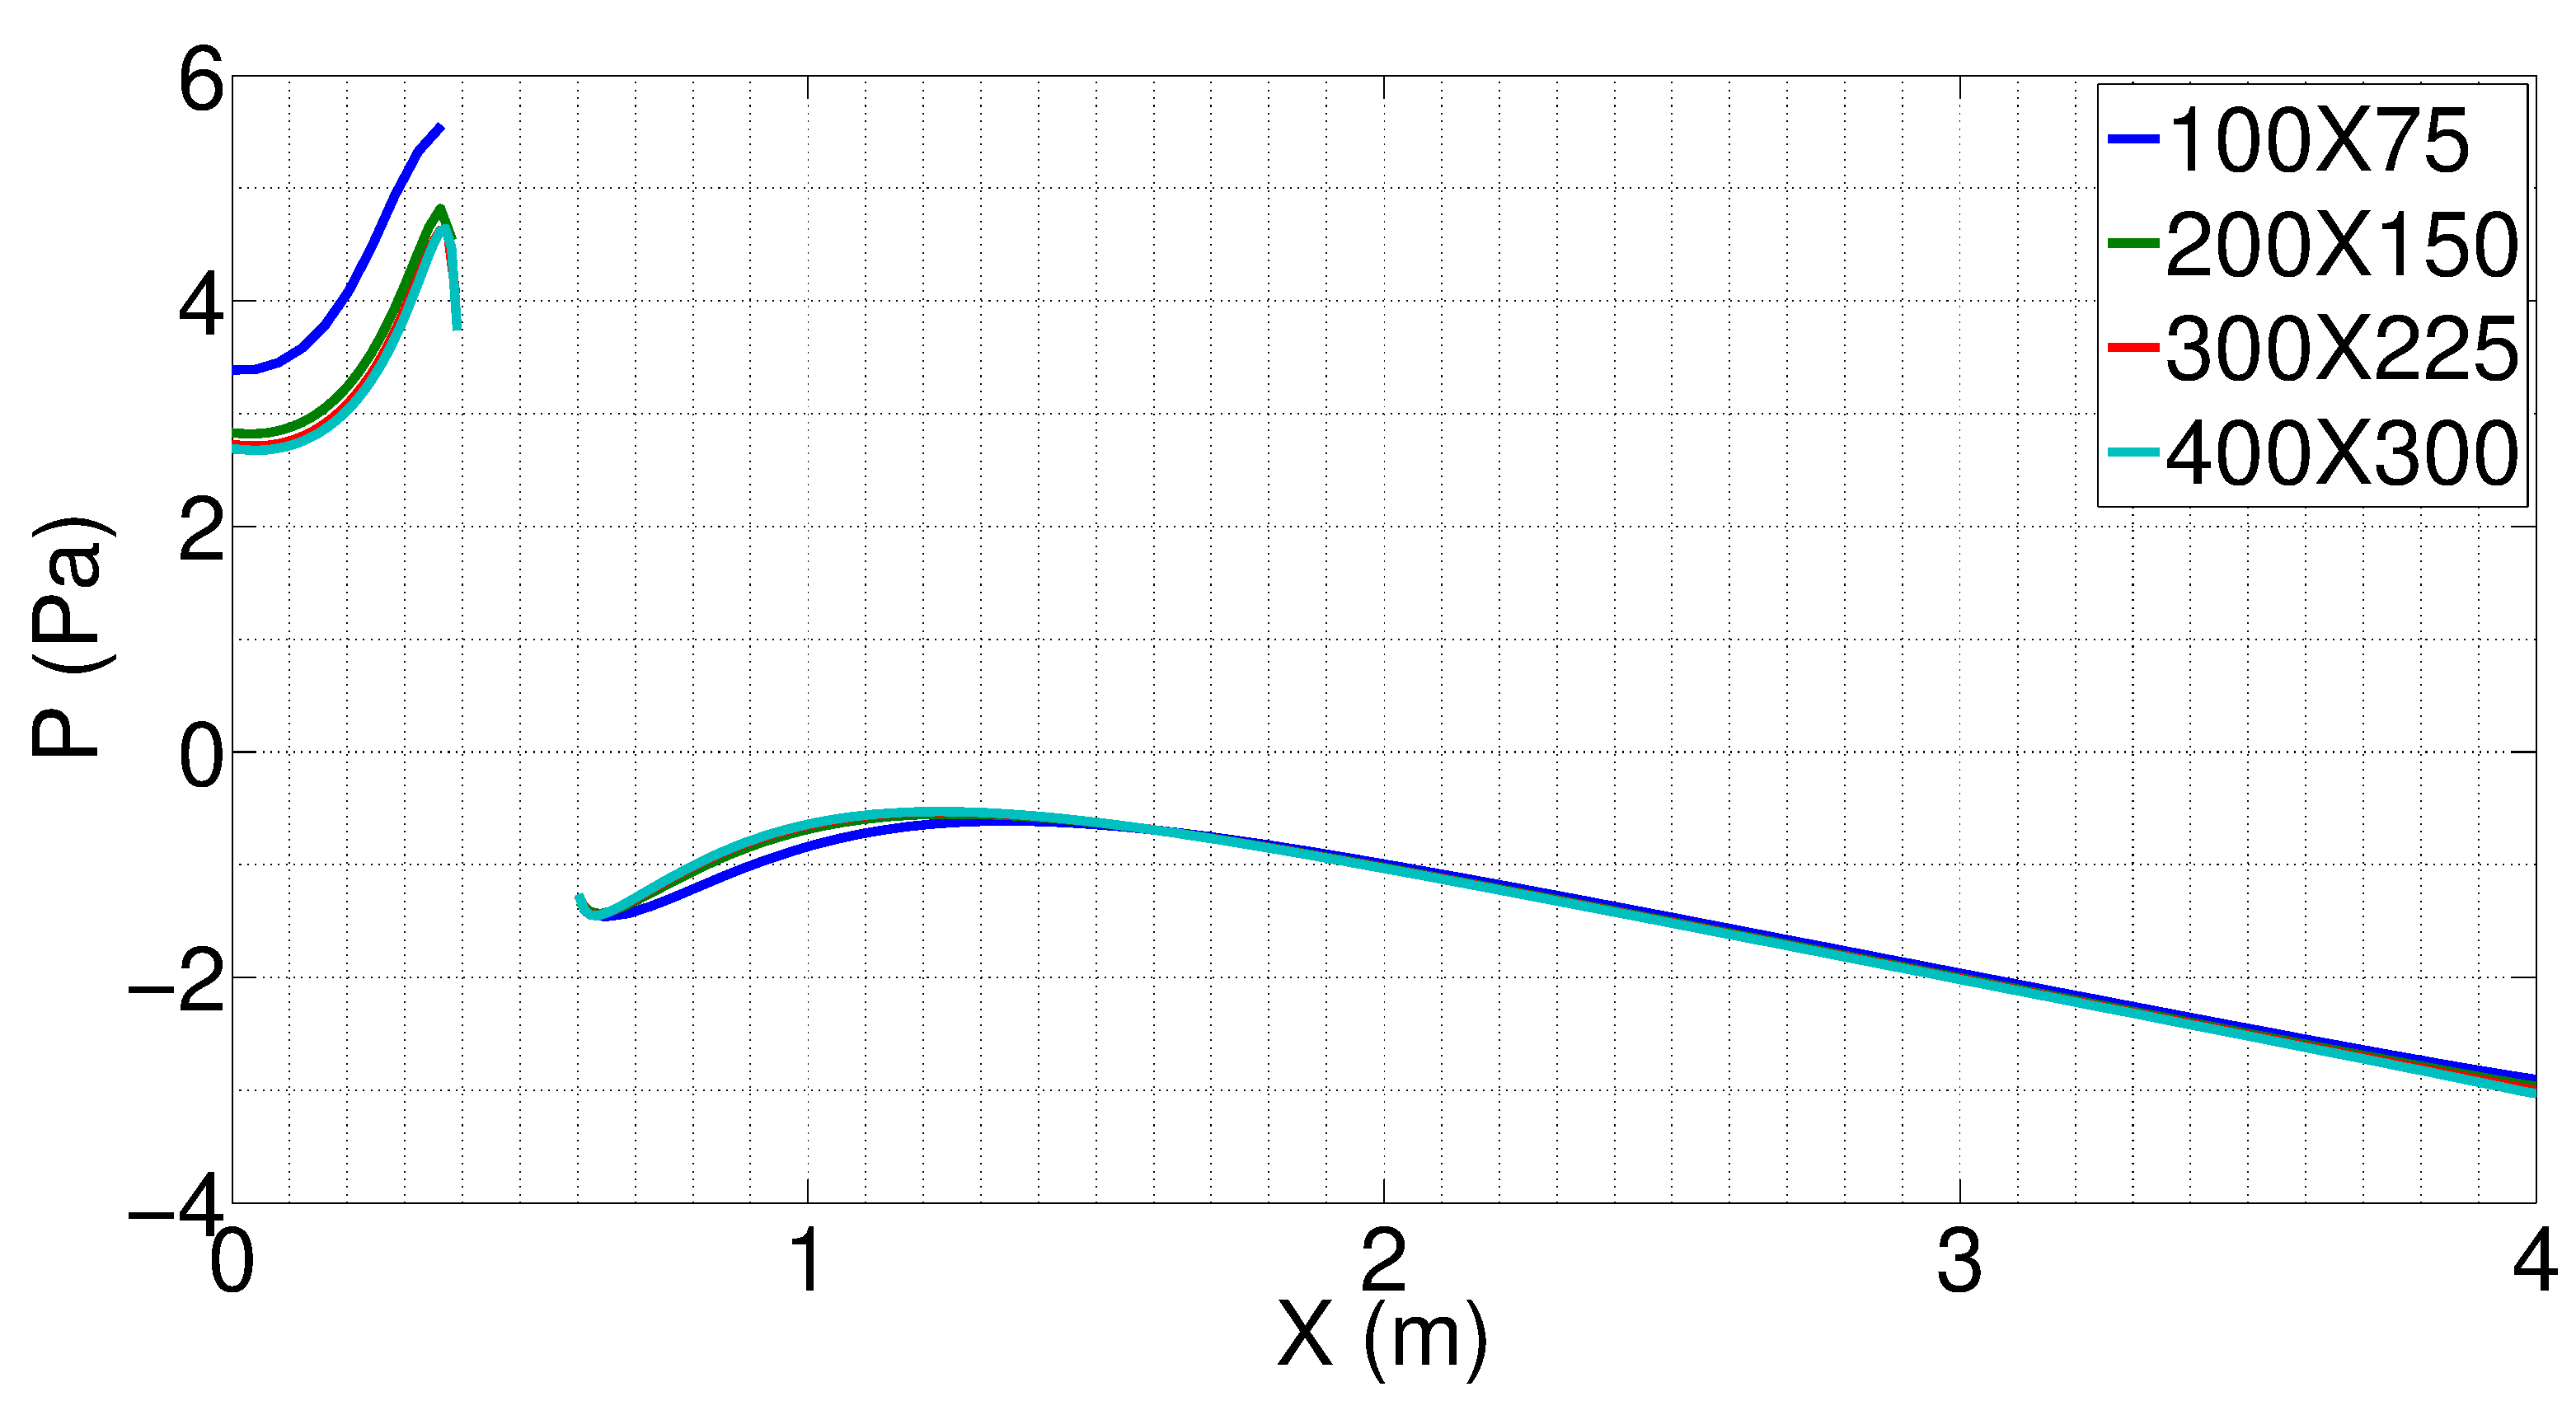
\includegraphics[width=7.0cm]{Chapter_4/figure/flow_over_cylinder/meshConvergence_RE100_P.eps}
    }
    \caption{Convergence results for Re = 100.}
    \label{fig:C4_meshConvergenceForCylidnerRE100GE}
\end{figure}

The convergence study of the mesh refinement is also conducted for a node on the downwash of the cylinder at $(2, 0)$ as shown in Figure \ref{fig:C4_meshRefinementForCylinderRE100GE}. The slopes of the fitted lines to the u-velocity, v-velocity, and pressure error estimates are calculated as $-2.34$, and $-1.96$, and $-2.72$. This means that the method is second order in space and time.

\begin{figure}[H]
    \centering
    \subfigure[U-velocity convergence on $(2.0, 0)$.]
    {
    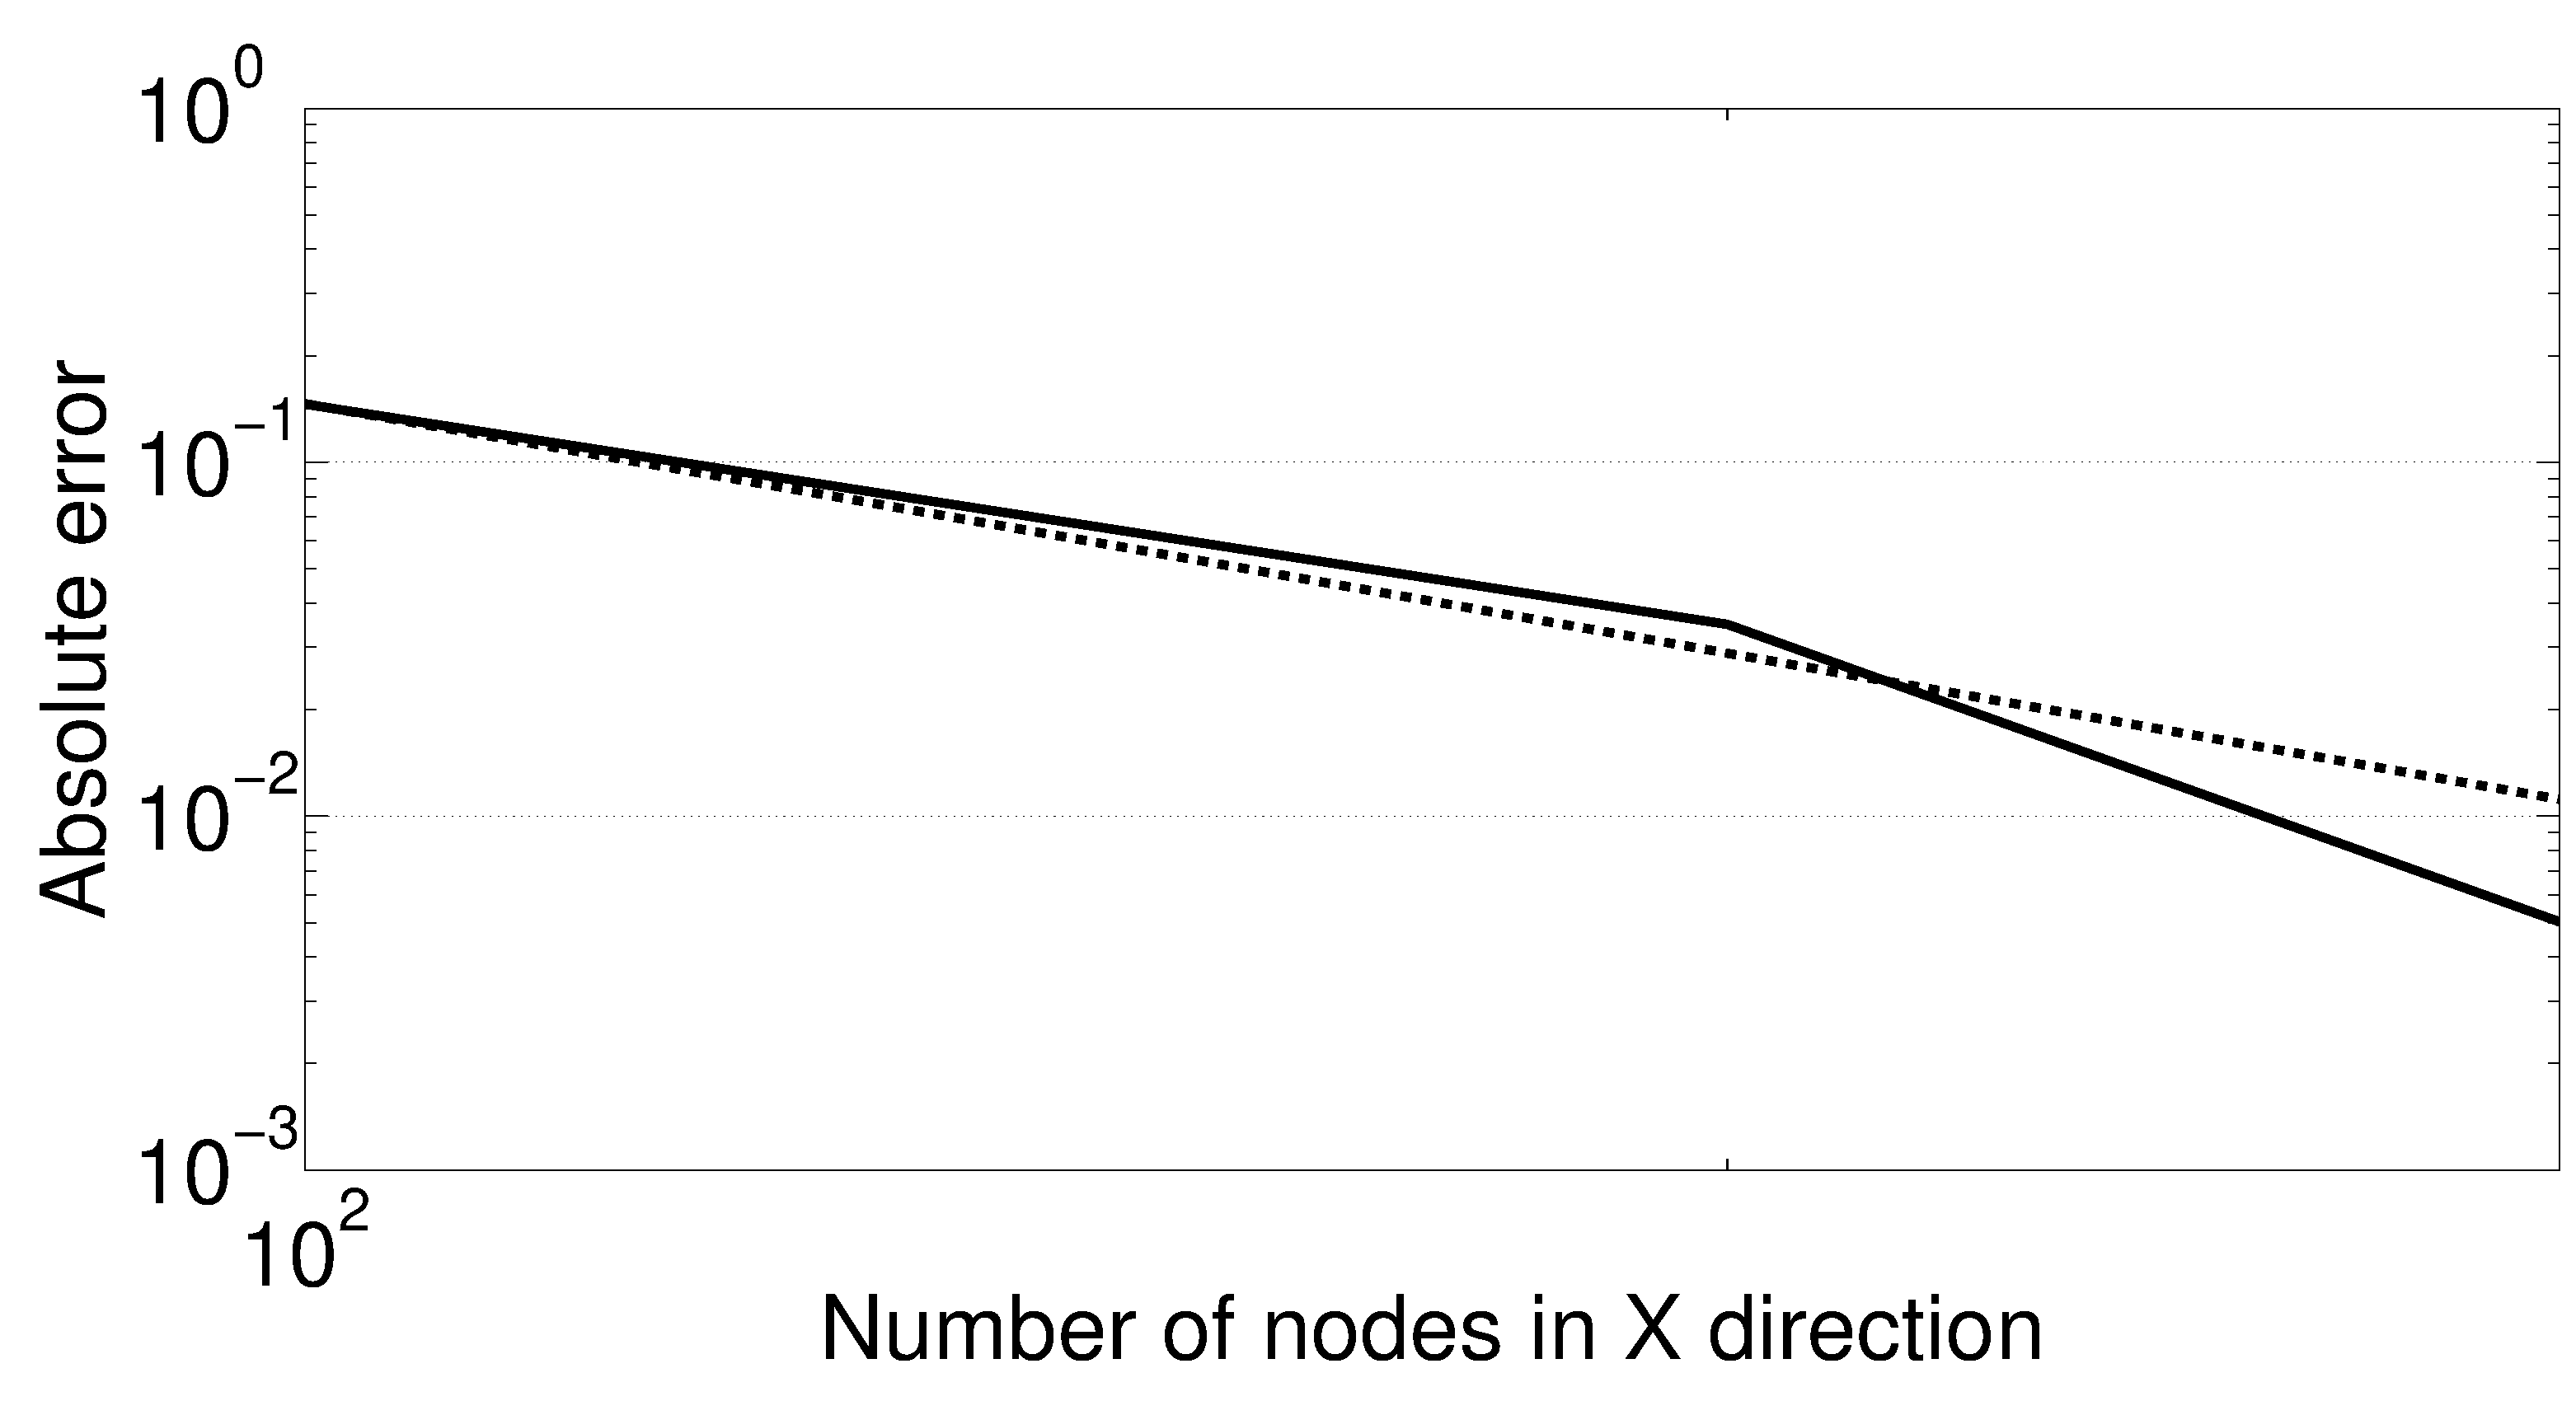
\includegraphics[width=7.0cm]{Chapter_4/figure/flow_over_cylinder/u_convergence_RE100.eps}
    }
    \quad
    \subfigure[V-velocity convergence on $(0.5, 0.75)$.]
    {
    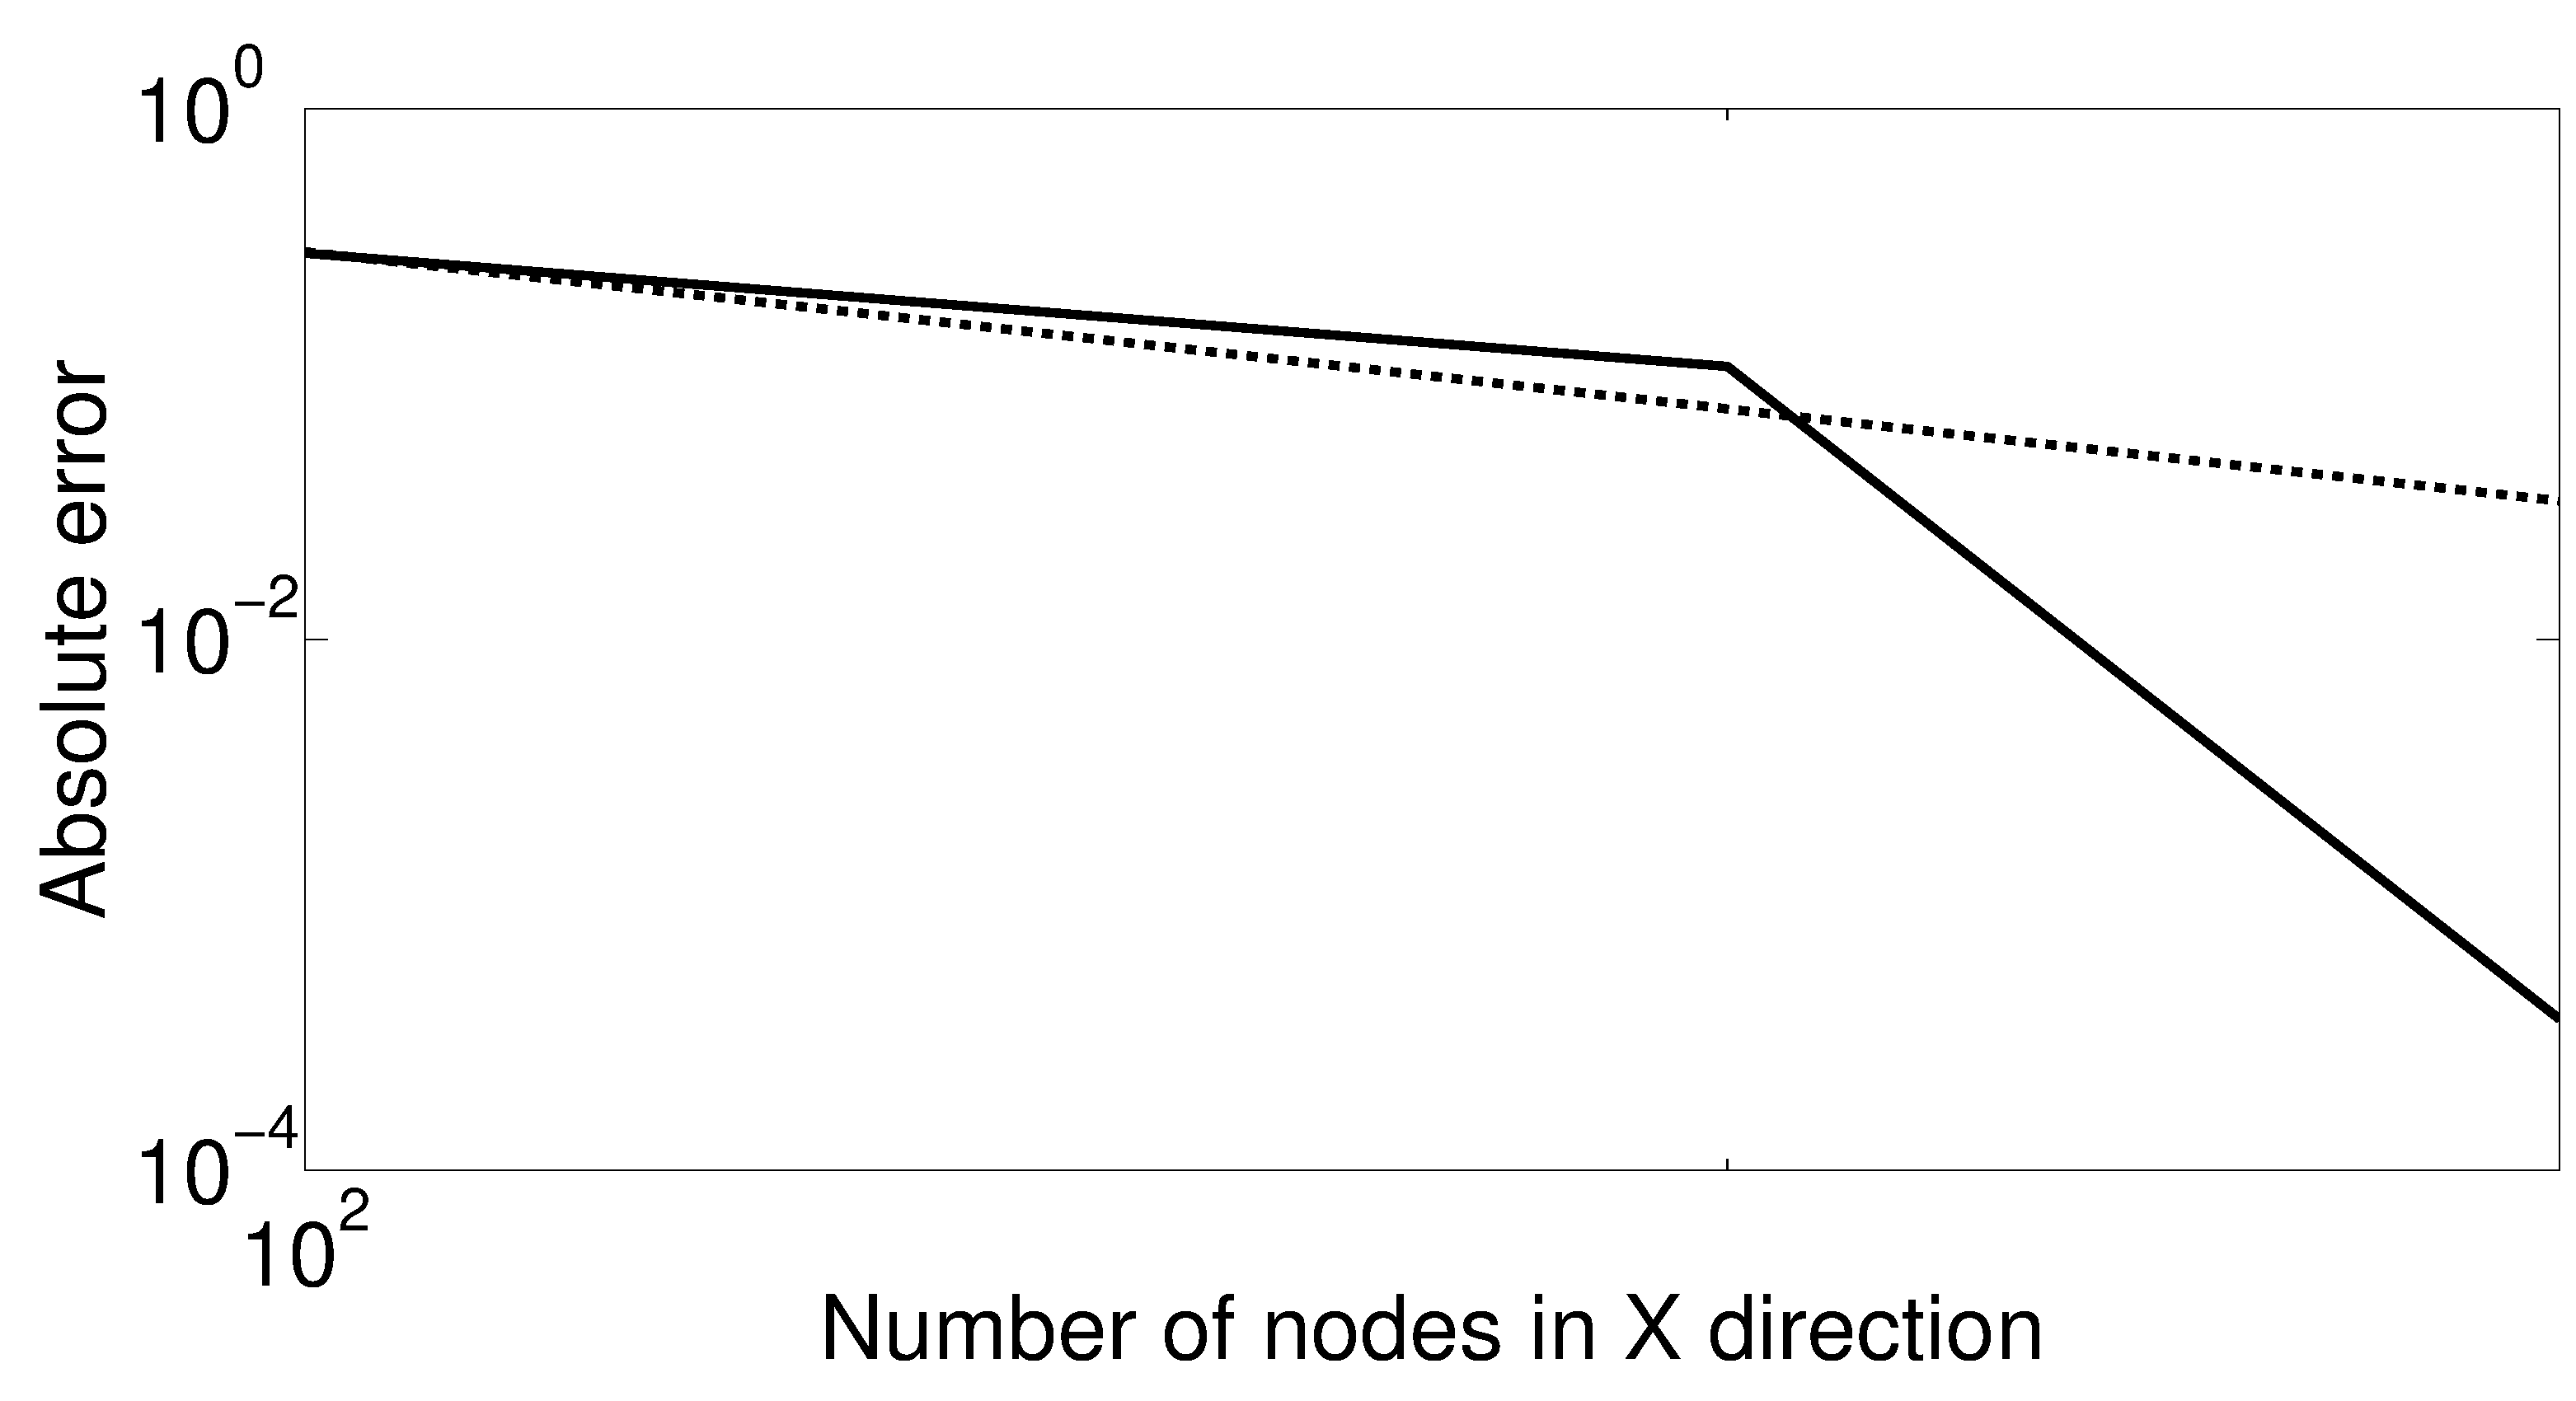
\includegraphics[width=7.0cm]{Chapter_4/figure/flow_over_cylinder/v_convergence_RE100.eps}
    }
    \\
    \subfigure[Pressure convergence on $(2.0, 0)$.]
    {
    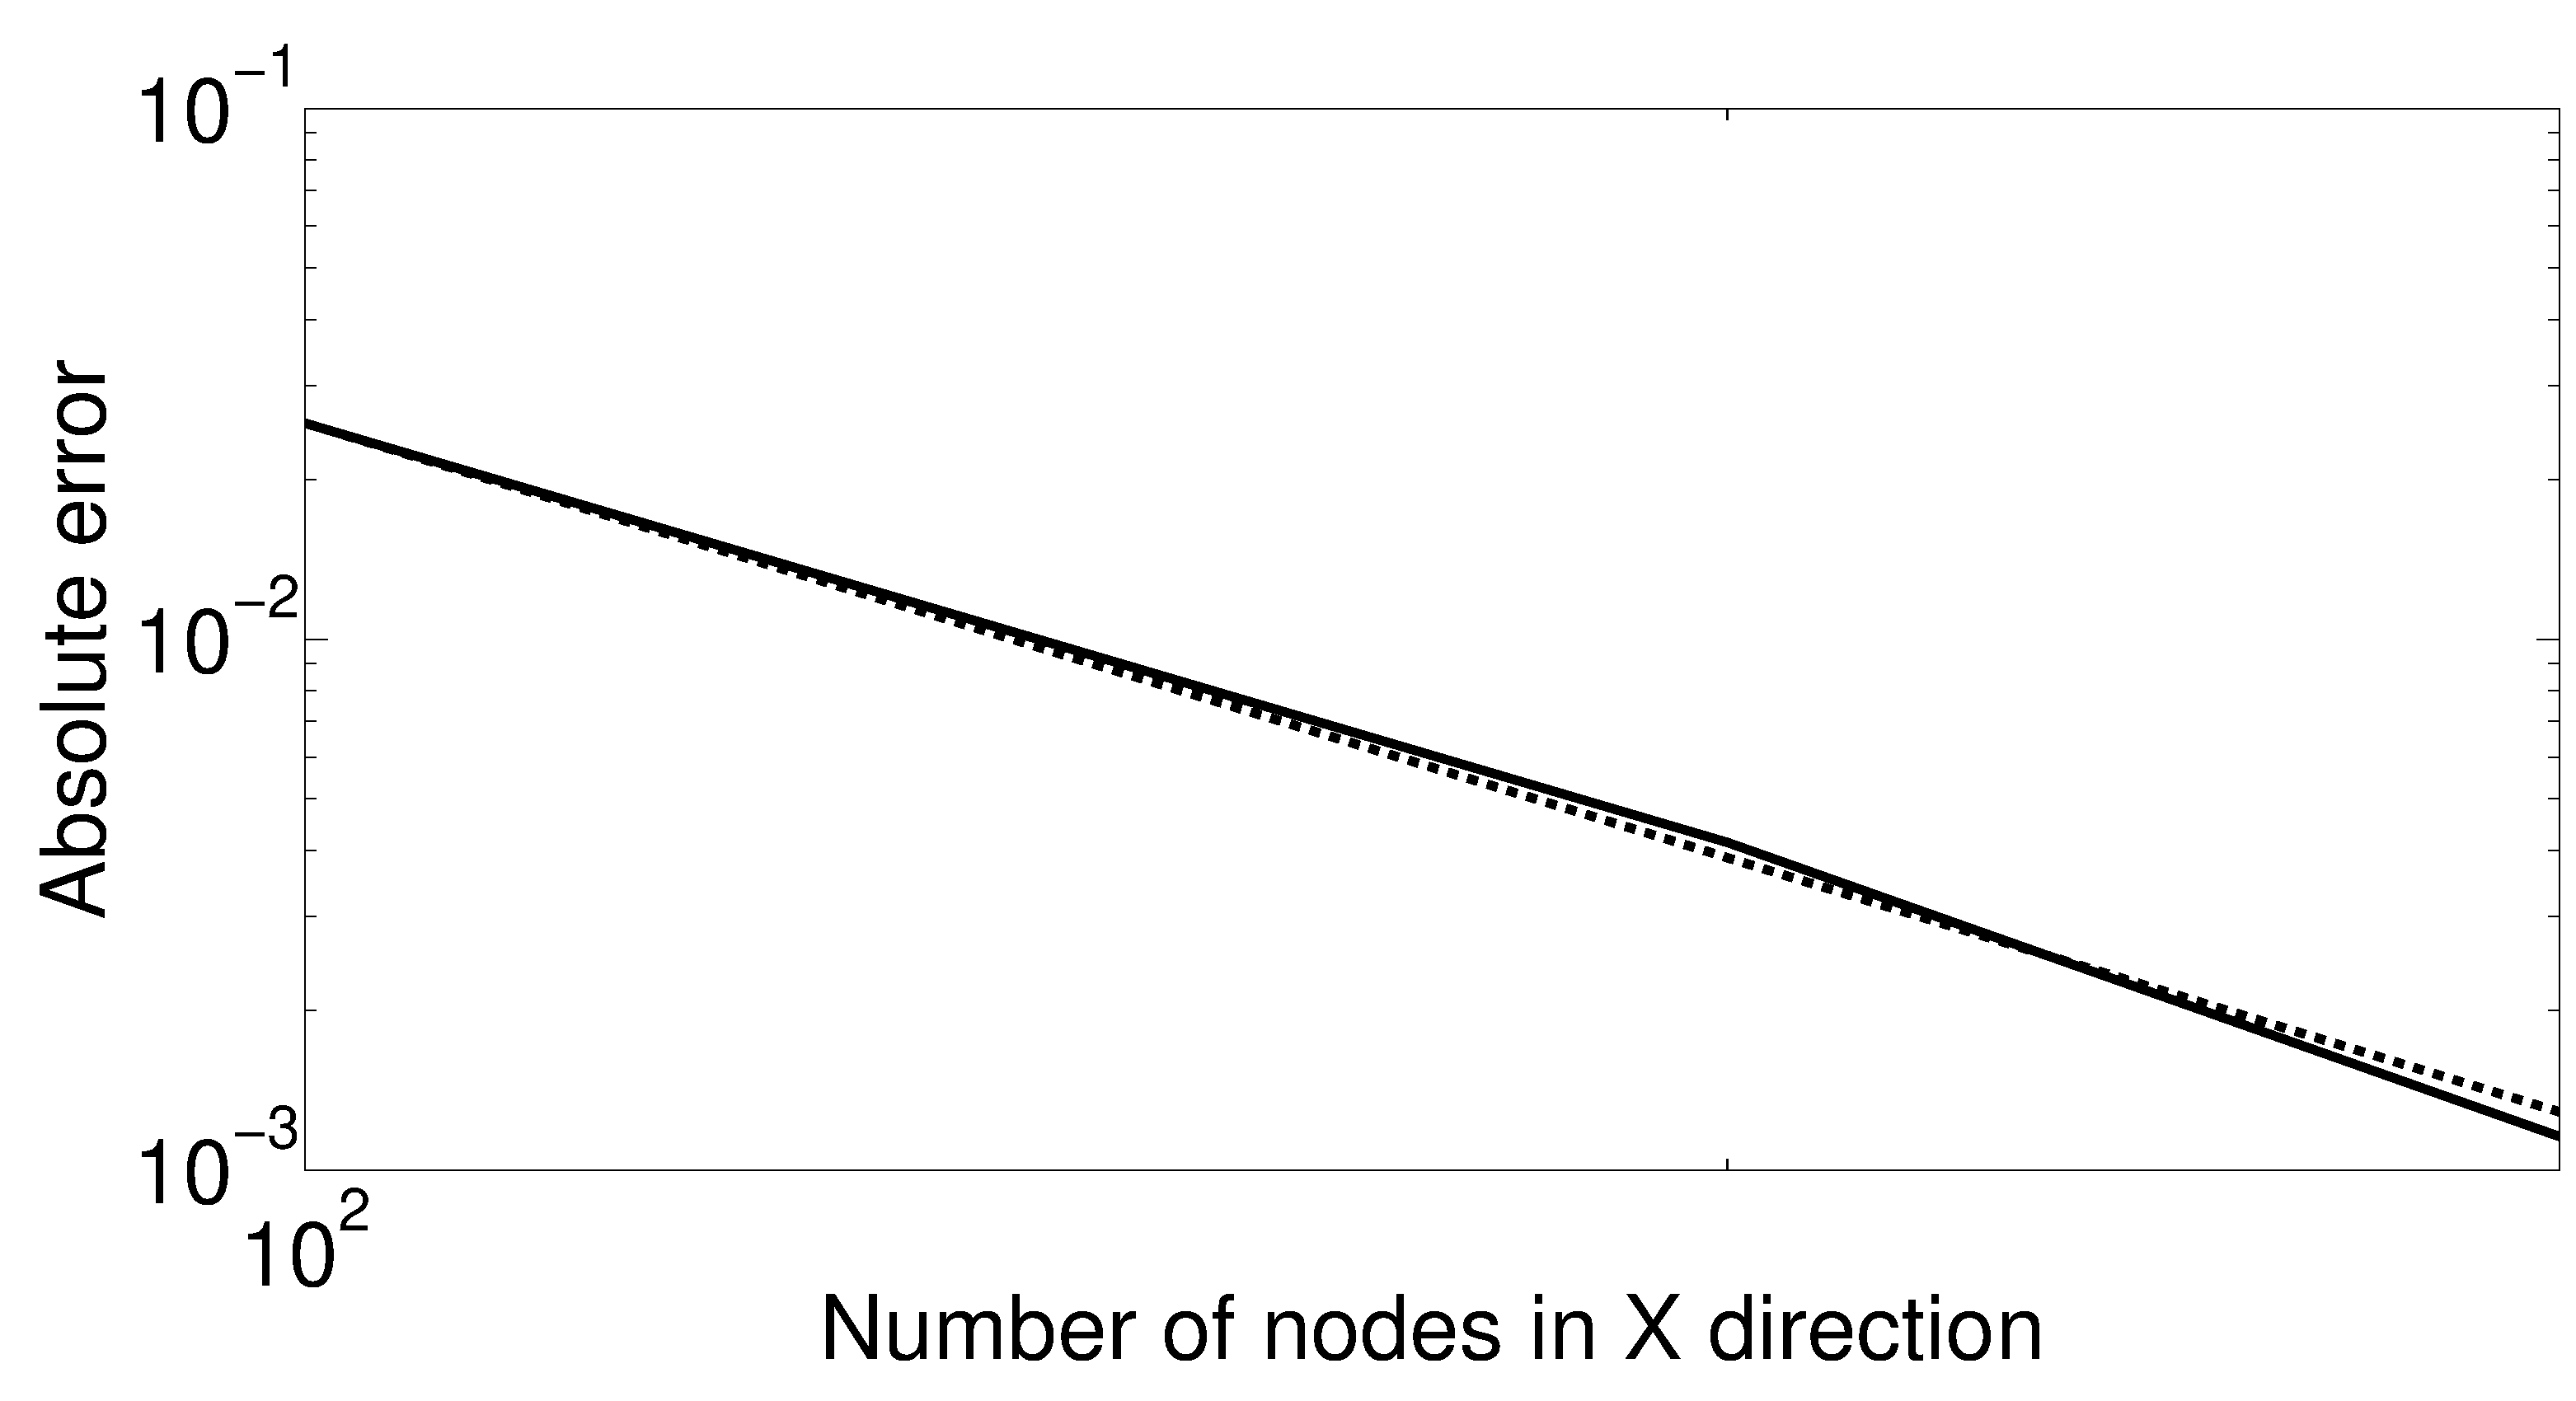
\includegraphics[width=7.0cm]{Chapter_4/figure/flow_over_cylinder/pressure_convergence_RE100.eps}
    }
    \caption{Convergence plots for Re = 100.}
    \label{fig:C4_meshRefinementForCylinderRE100GE}
\end{figure}

The contour plots for the velocity and pressure is shown in Figure \ref{fig:C4_contourPlotsForFlowOverCylidnerGE}.

\begin{figure}[H]
    \centering
    \subfigure[U-velocity]
    {
    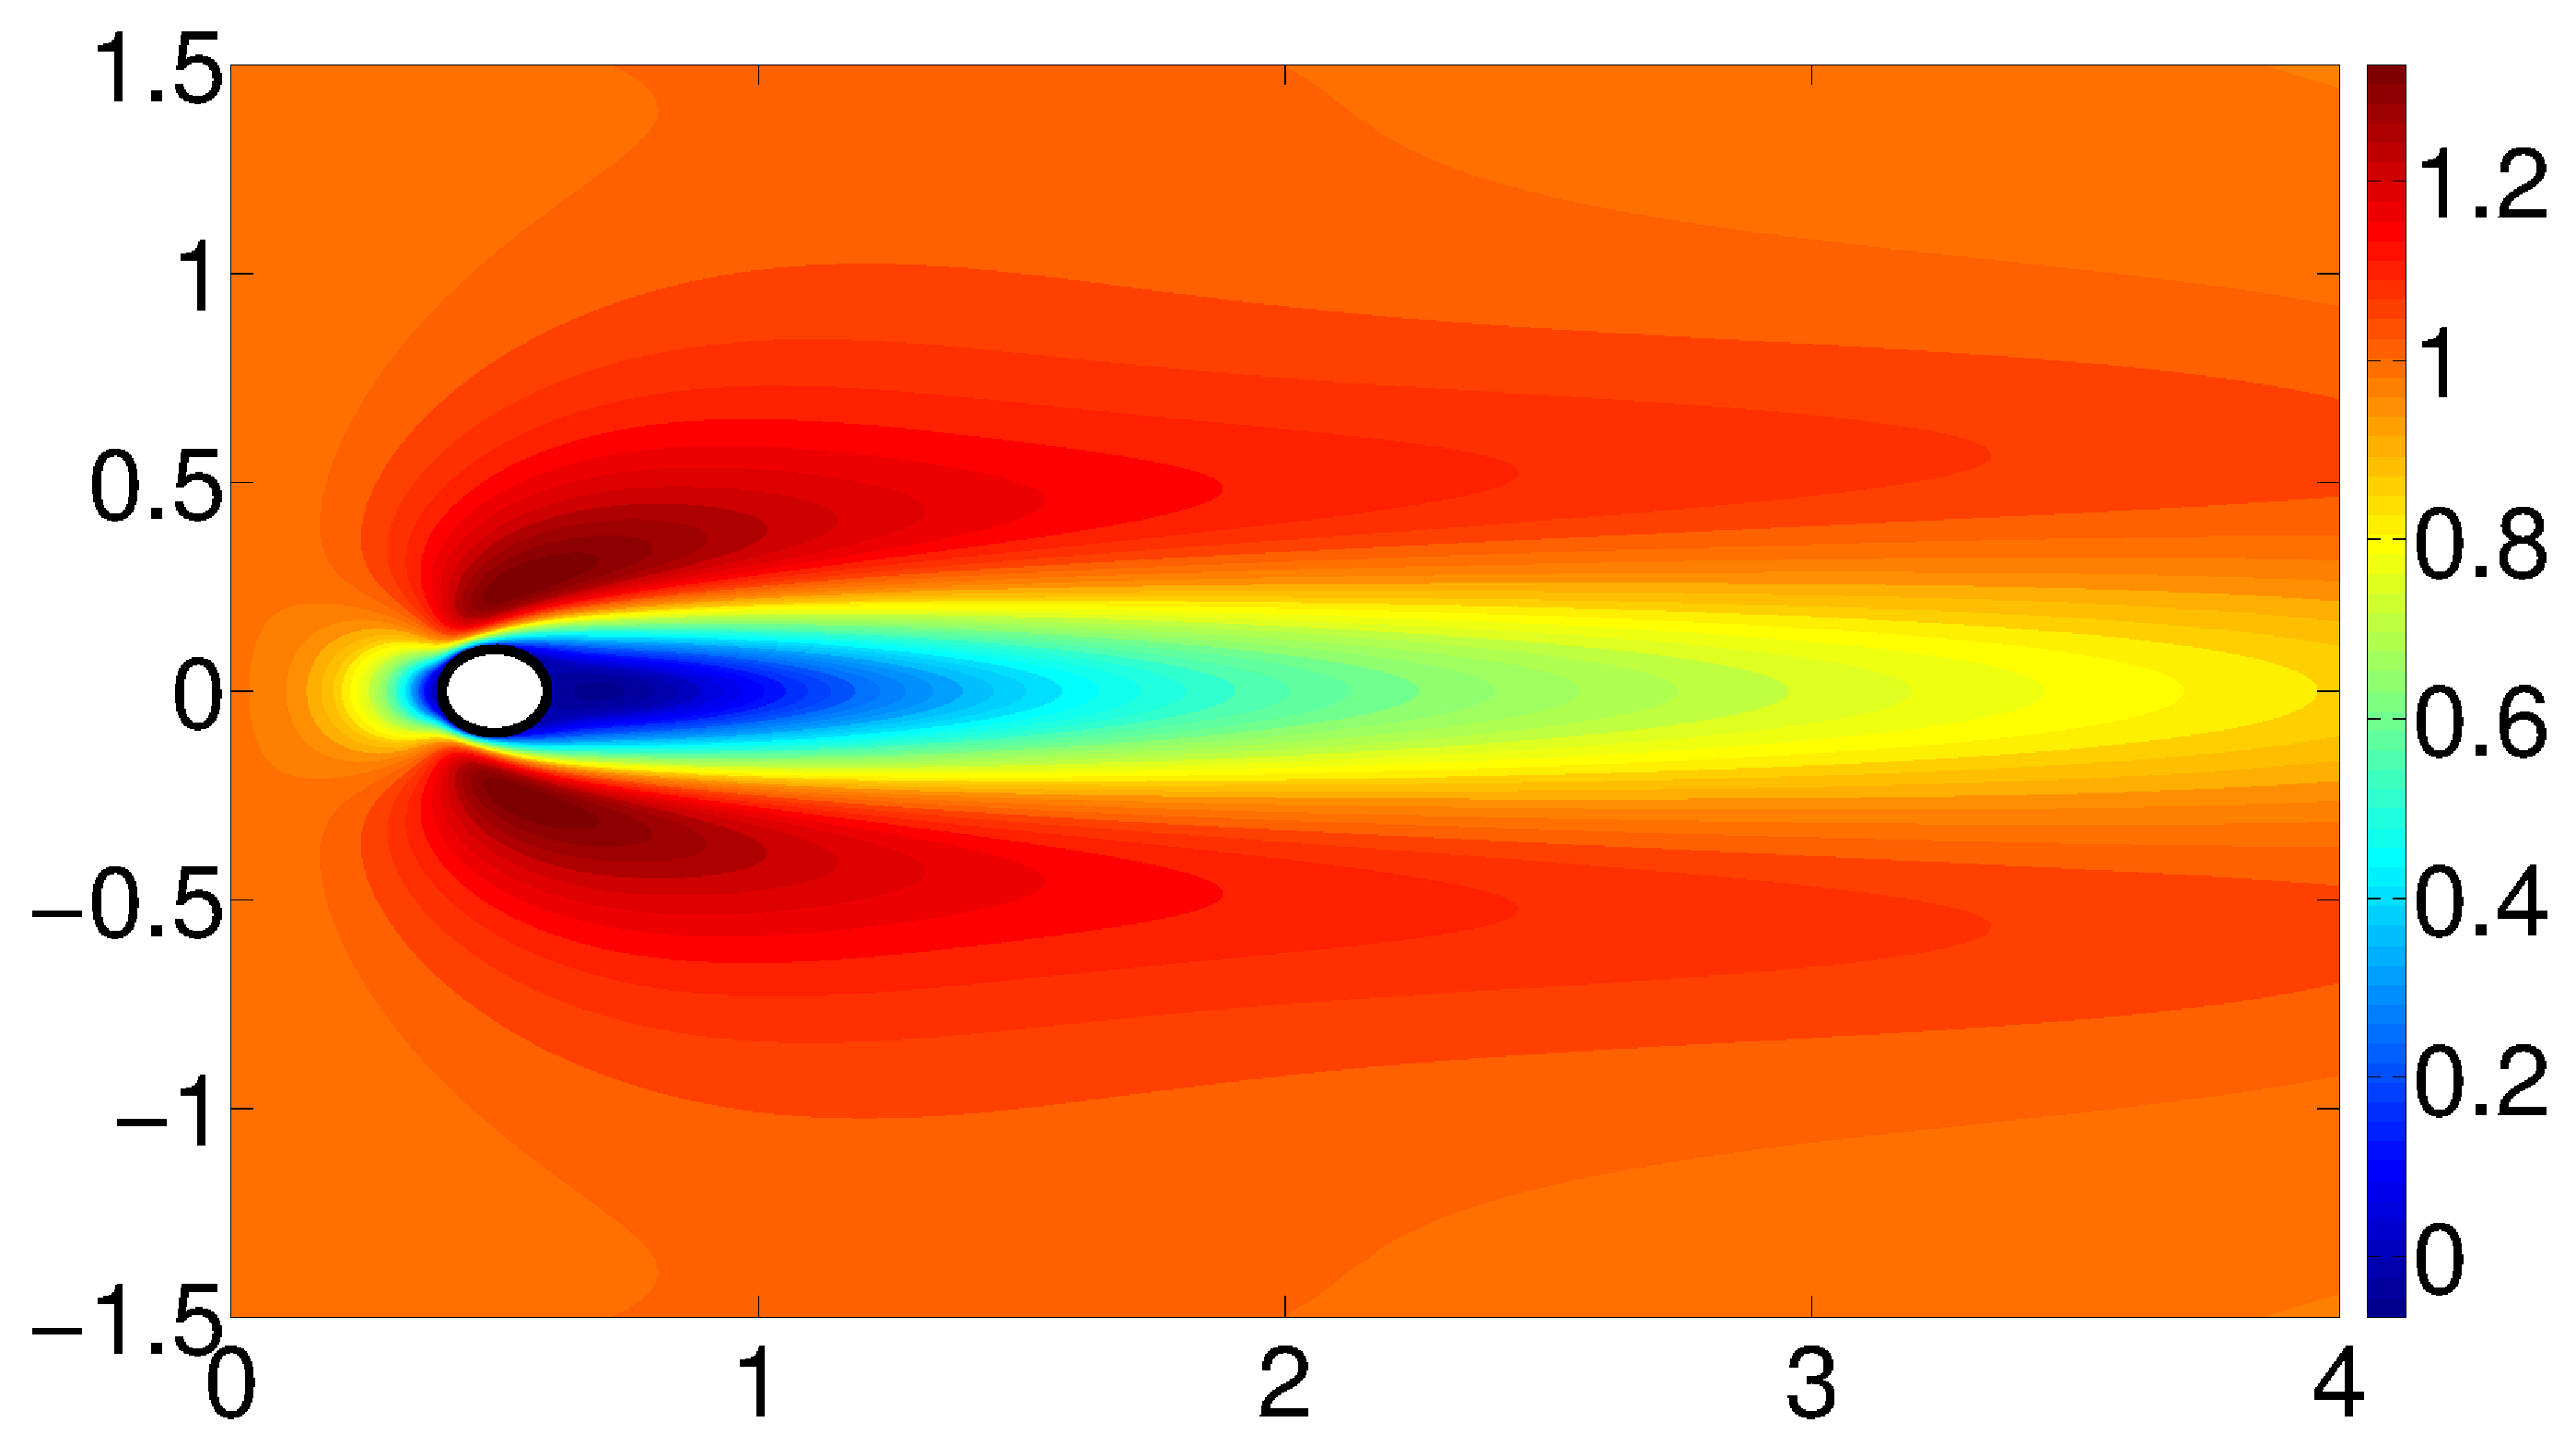
\includegraphics[width=7.0cm]{Chapter_4/figure/flow_over_cylinder/u_velocity_contour_RE100.eps}
    }
    \quad
    \subfigure[V-velocity]
    {
    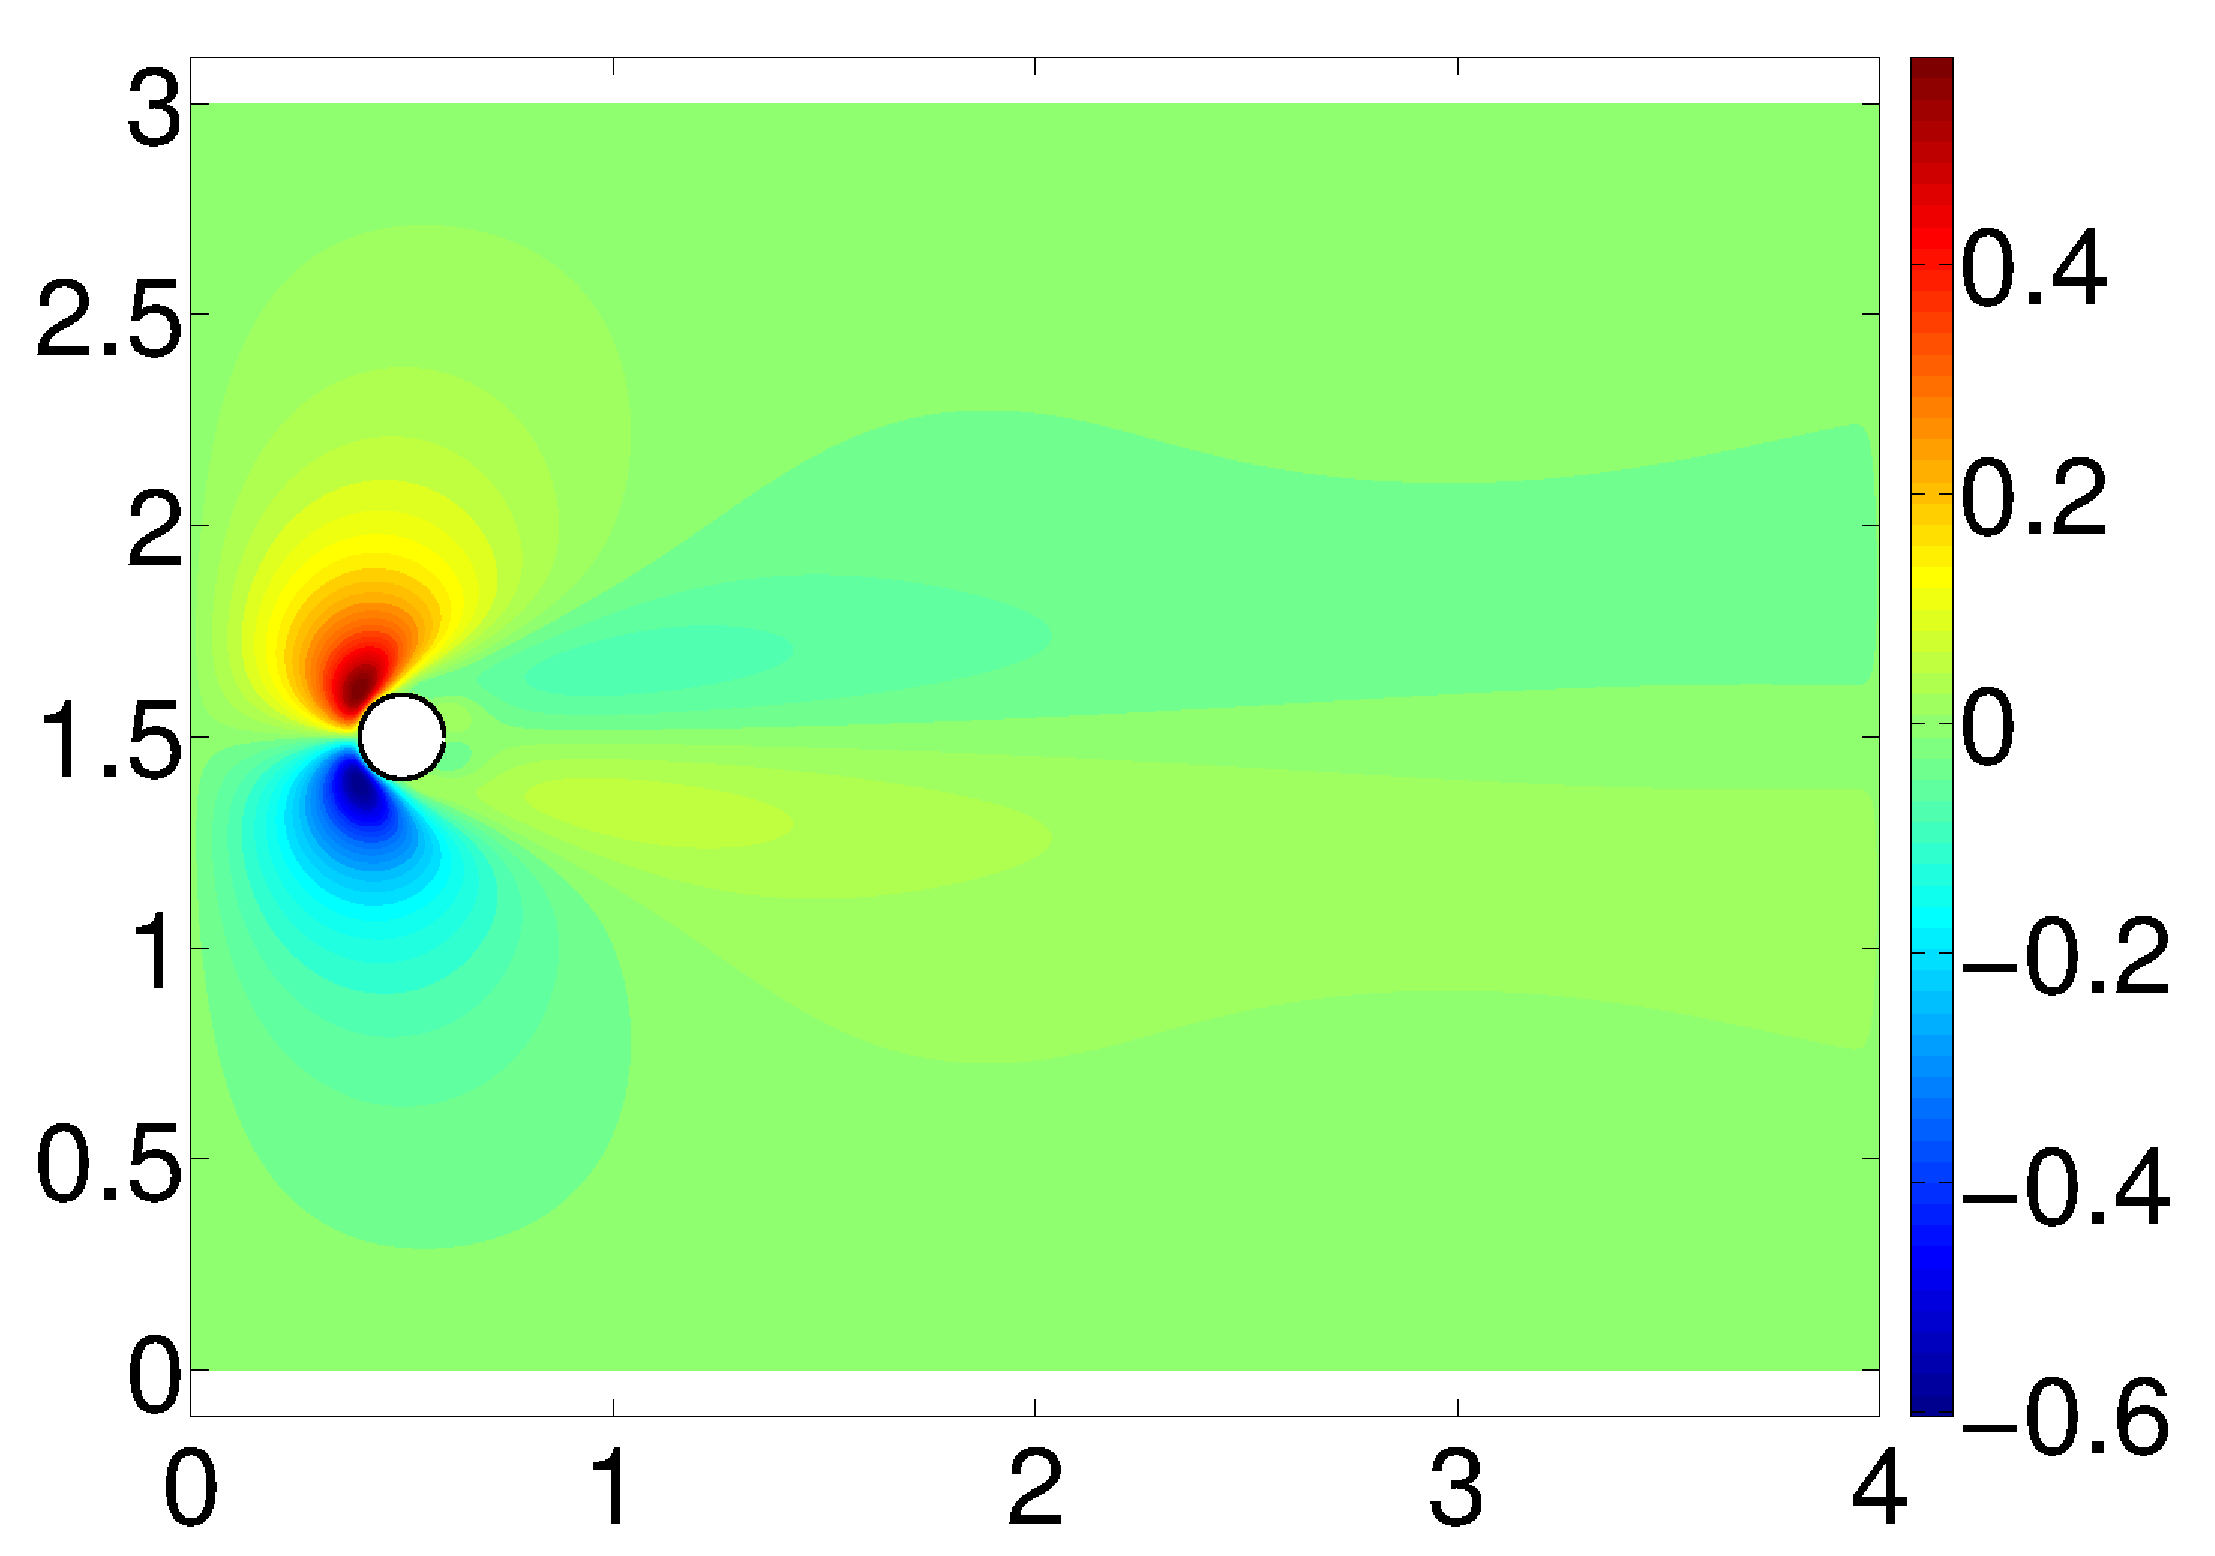
\includegraphics[width=7.0cm]{Chapter_4/figure/flow_over_cylinder/v_velocity_contour_RE100.eps}
    }
    \caption{Velocity contours for Re = 100.}
    \label{fig:C4_contourPlotsForFlowOverCylidnerGE}
\end{figure}

To ensure that the zero velocity on the solid boundary, we looked at the value of the u and v velocities at the Lagrangian points on the boundary. These are shown in Figure \ref{fig:C4_fluidVelocityOnCylinder}. As shown here, the forcing terms brought the velocity to zero within the accuracy requirement. The oscillation on the velocity magnitude is due to their small values. The $\theta$ is the polar coordinate on Lagragian points on the surface of the cylinder as shown in Figure \ref{fig:C4_cylinderPhysicalDomain}.

\begin{figure}[H]
    \centering
    \subfigure[U-velocity]
    {
    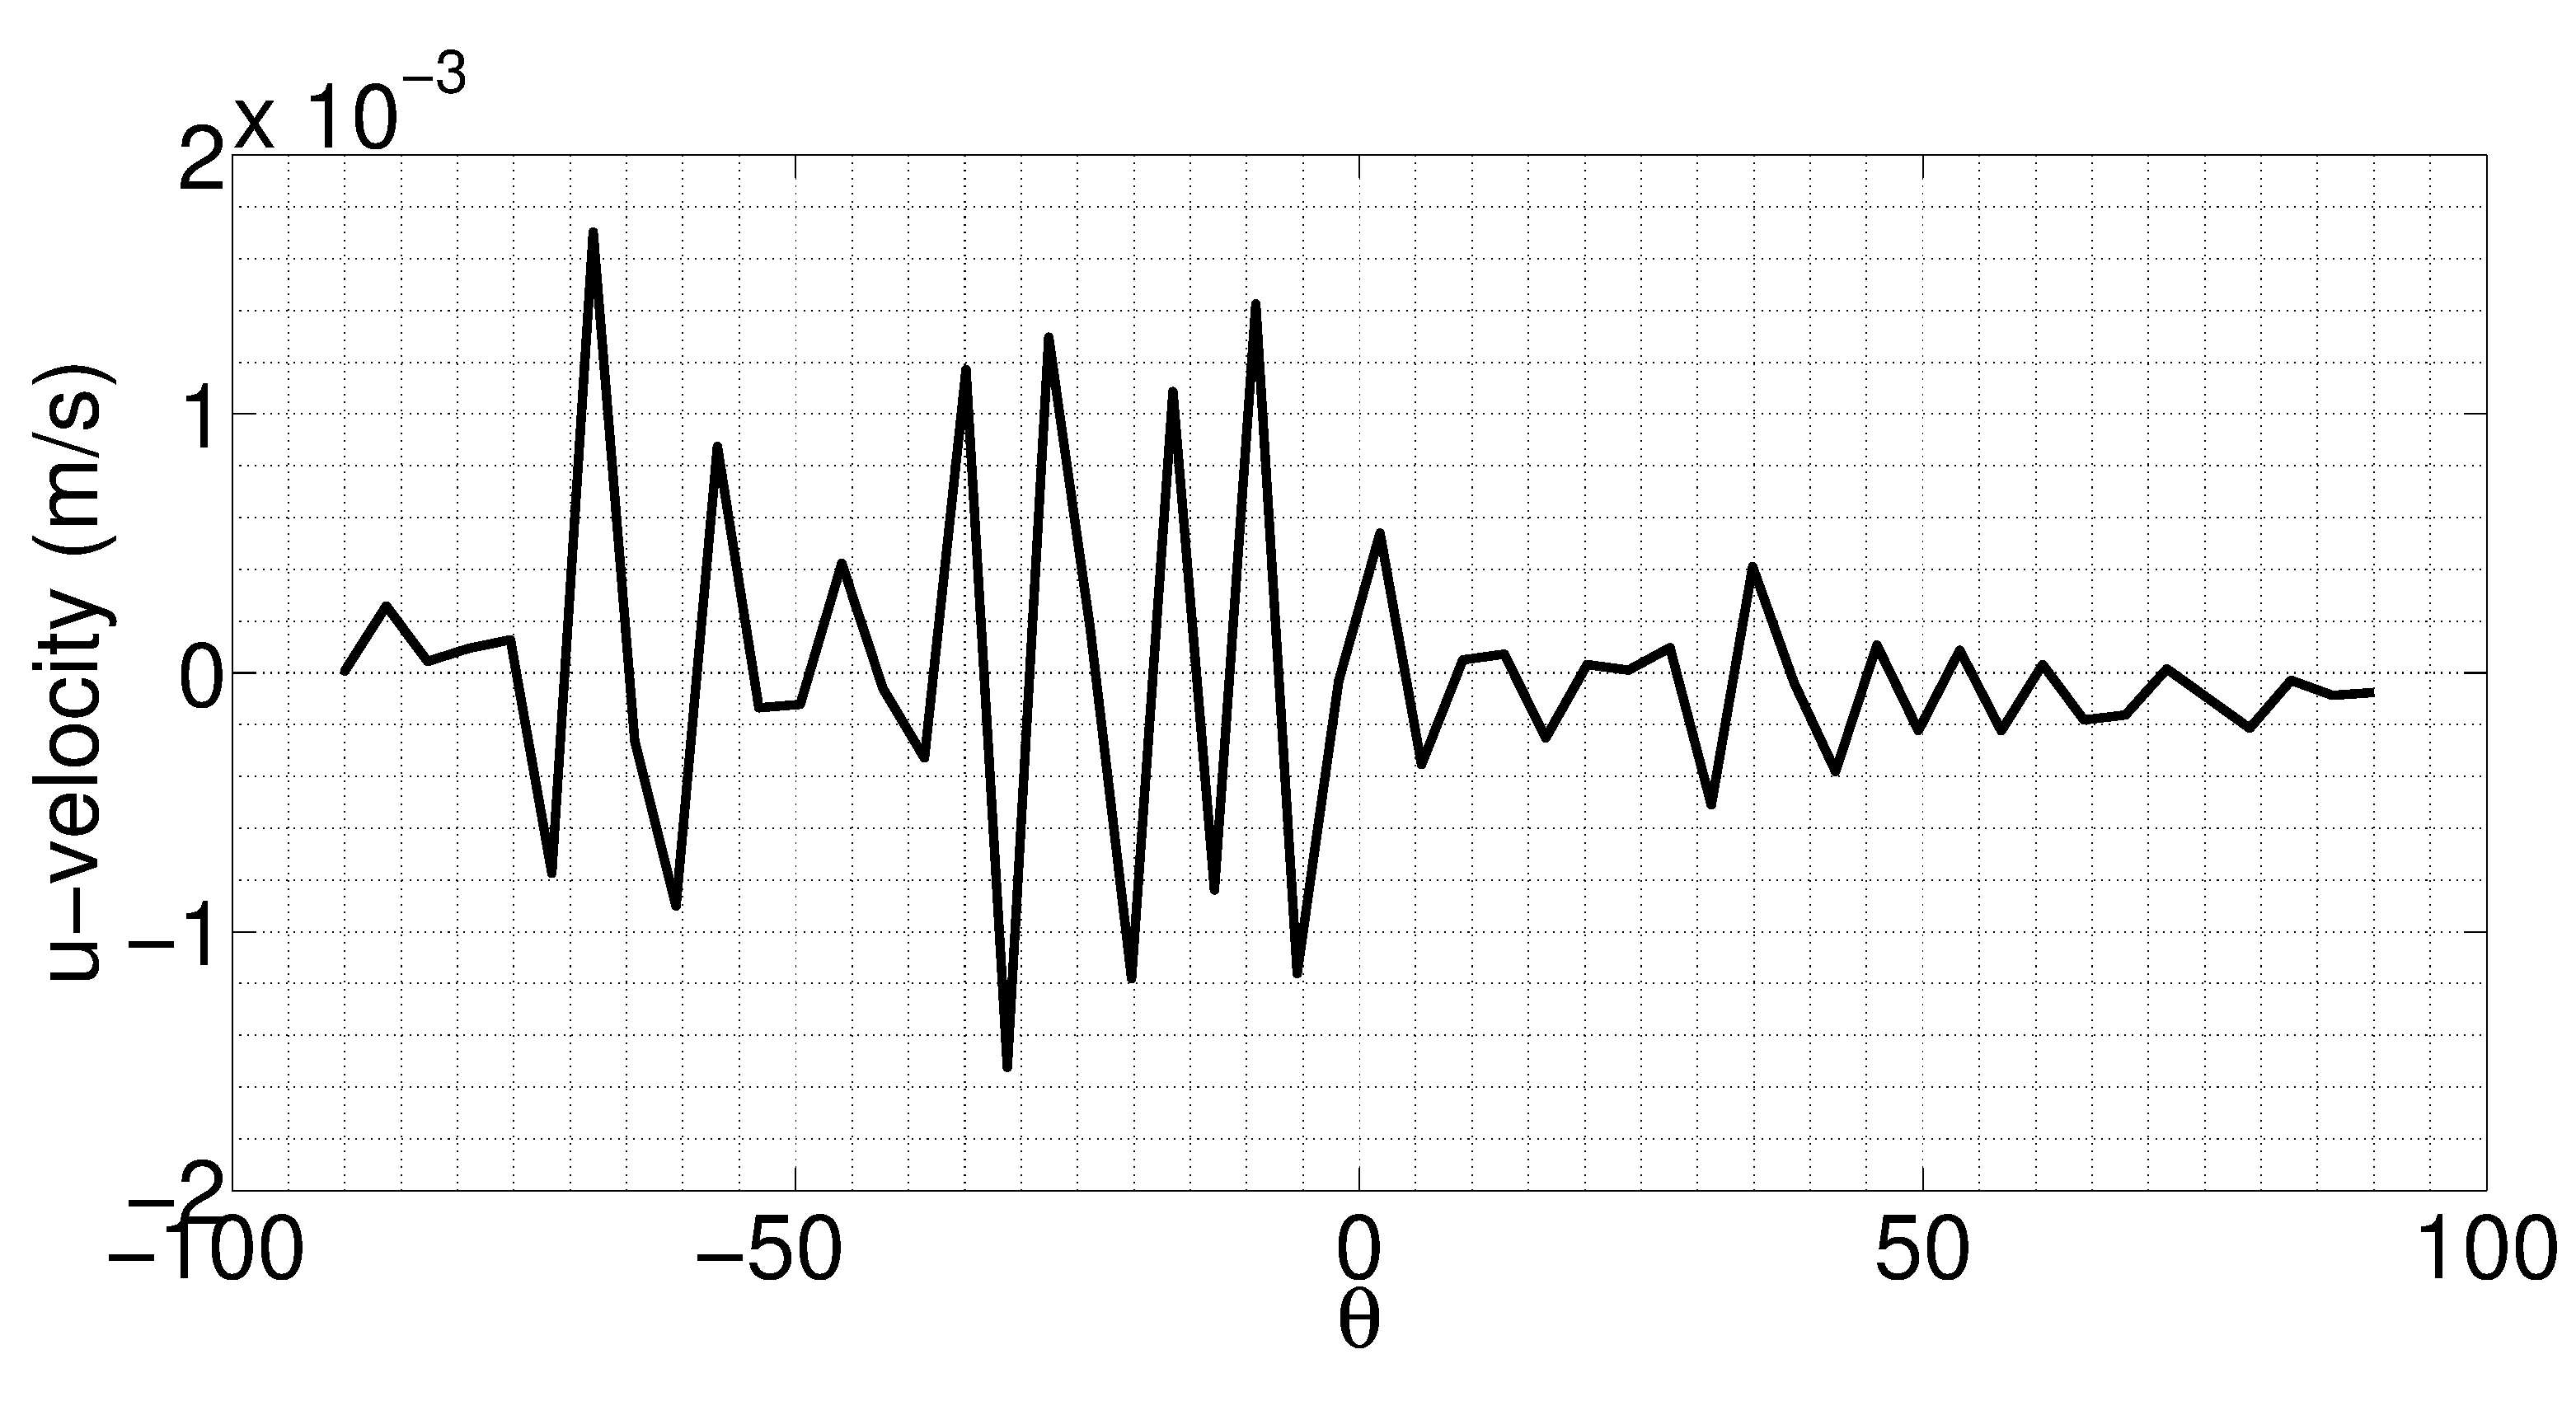
\includegraphics[width=7.0cm]{Chapter_4/figure/flow_over_cylinder/u_on_boundary_RE100.eps}
    }
    \quad
    \subfigure[V-velocity]
    {
    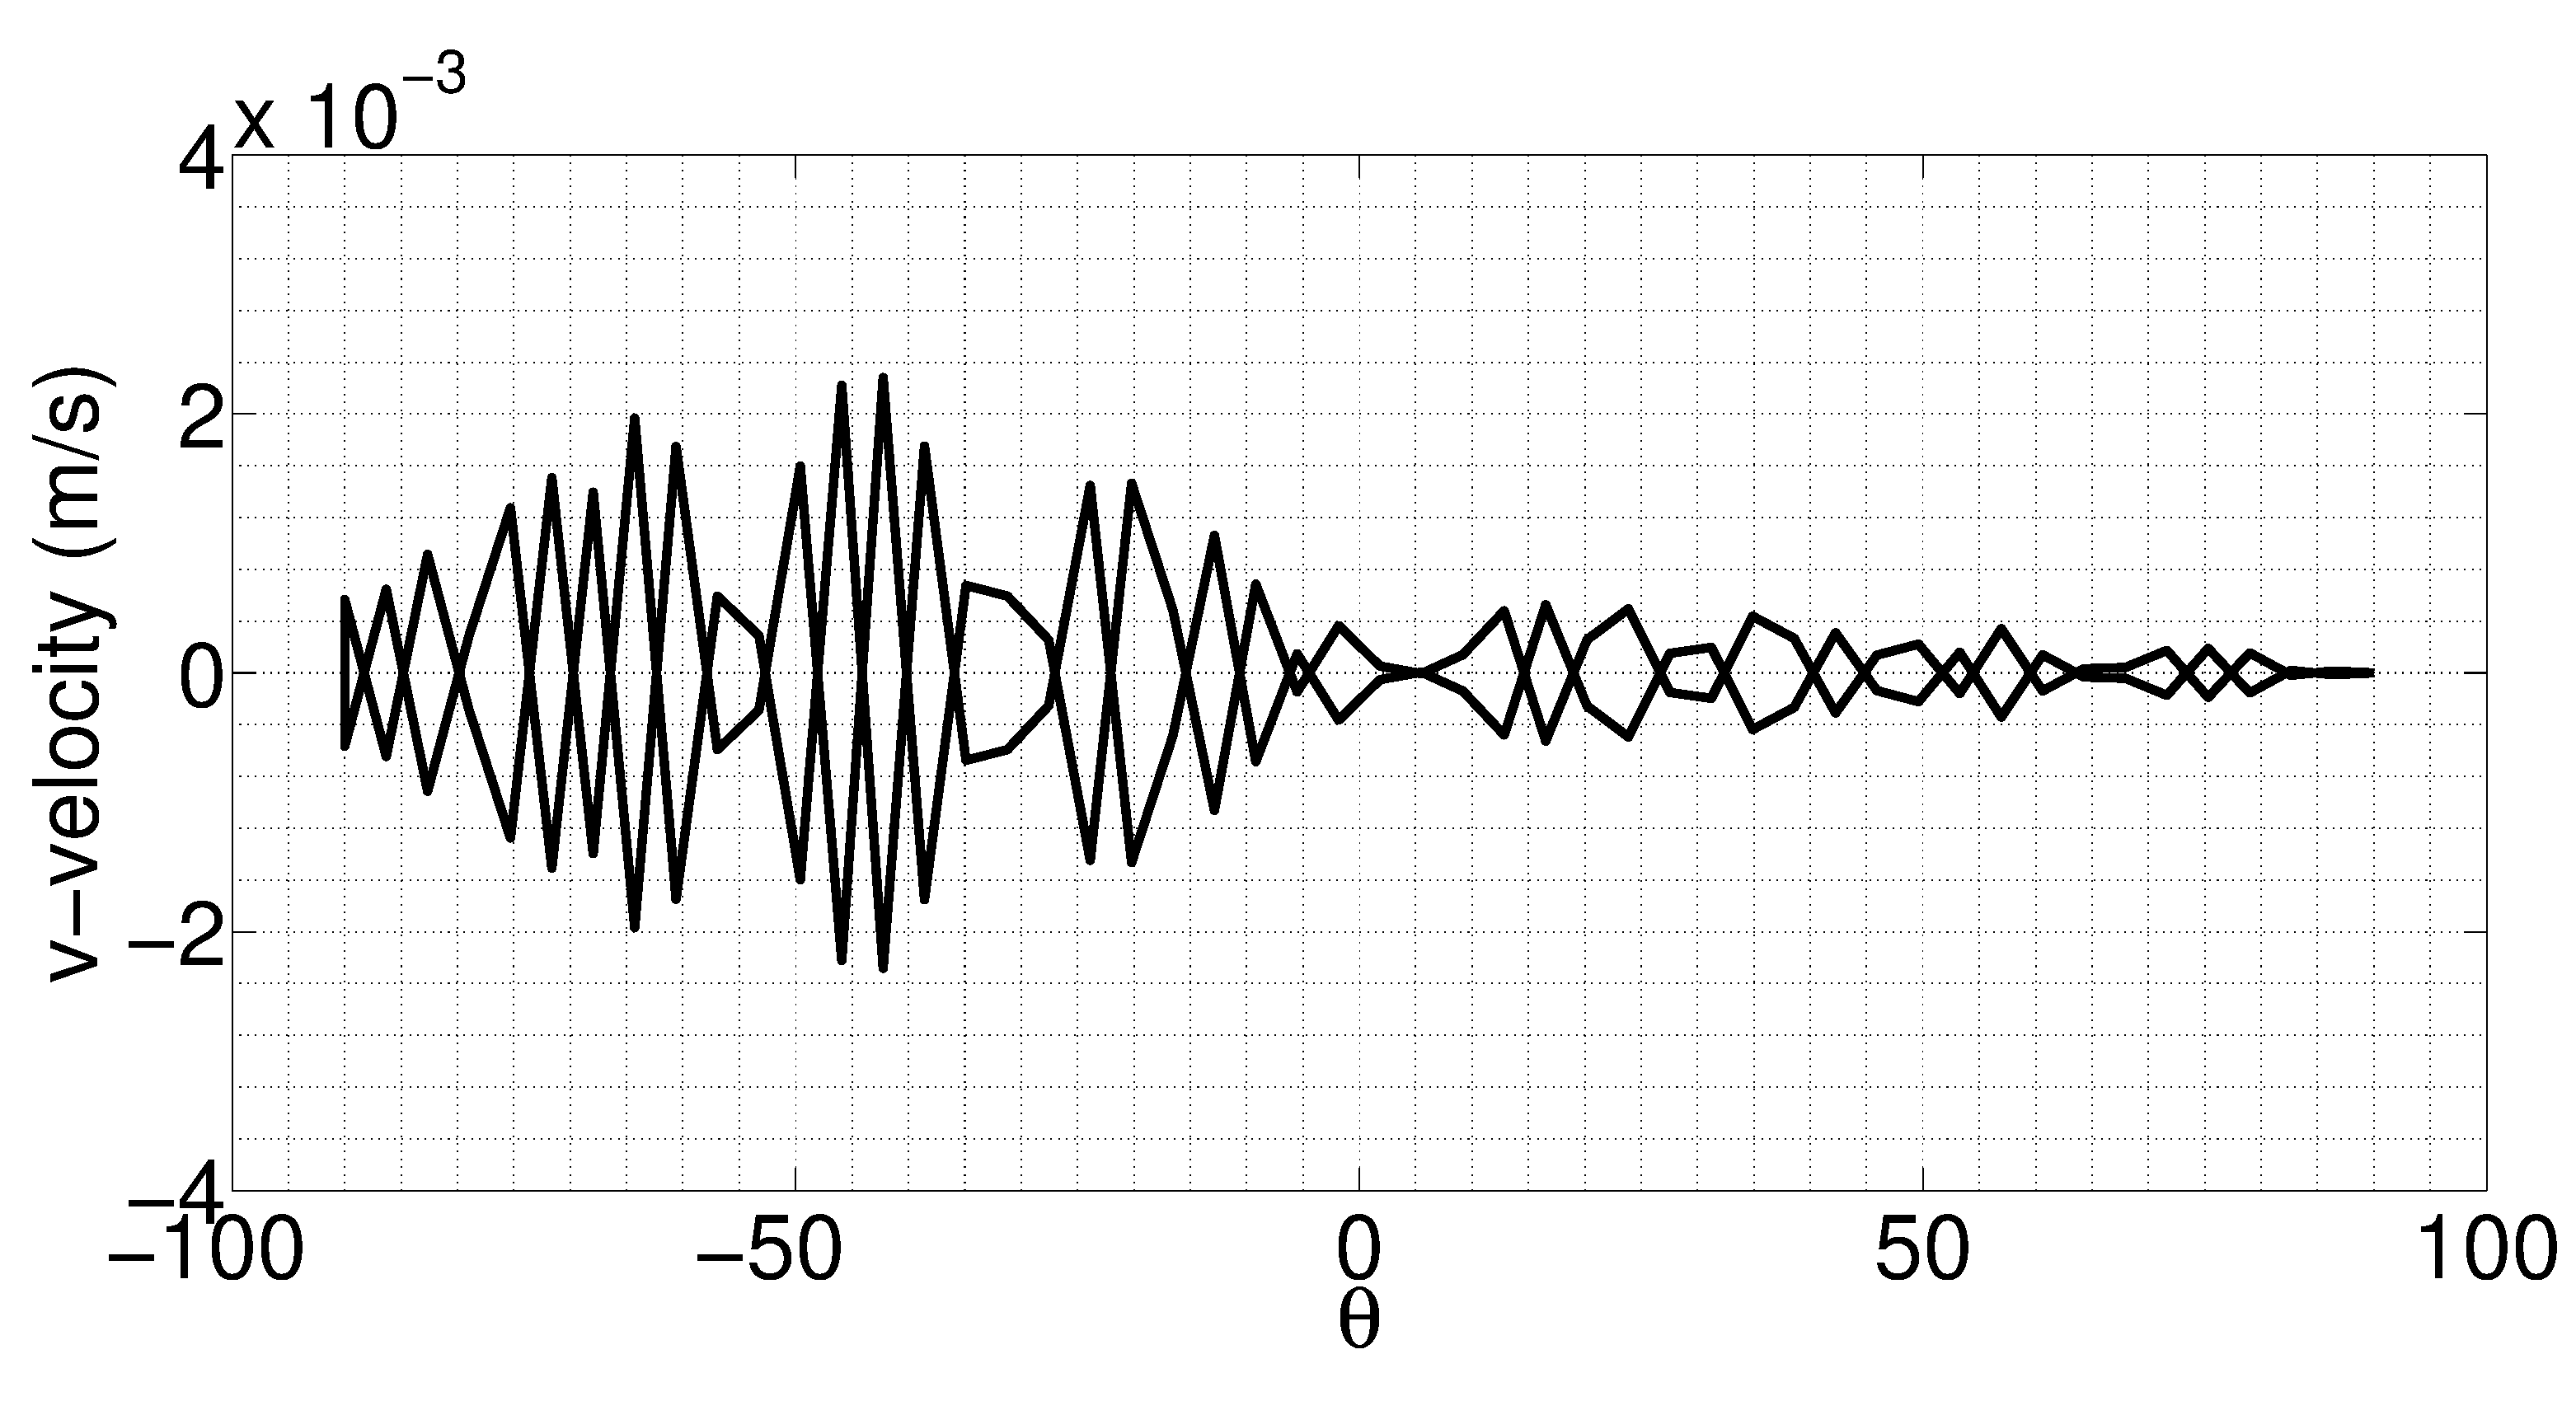
\includegraphics[width=7.0cm]{Chapter_4/figure/flow_over_cylinder/v_on_boundary_RE100.eps}
    }
    \caption{Velocity components on the solid boundary for Re = 100.}
    \label{fig:C4_fluidVelocityOnCylinder}
\end{figure}

Finally, the pressure profile on the surface of the cylinder is calculated as shown in Figure \ref{fig:C4_pressureOnSurfaceCylinder}. No smoothing is done for the calculating the pressure values on the Lagrangian points. This data is interpolated using the RD function of Equation \eqref{eq:C4_deltaFunction}.

\begin{figure}[H]
    \centering
    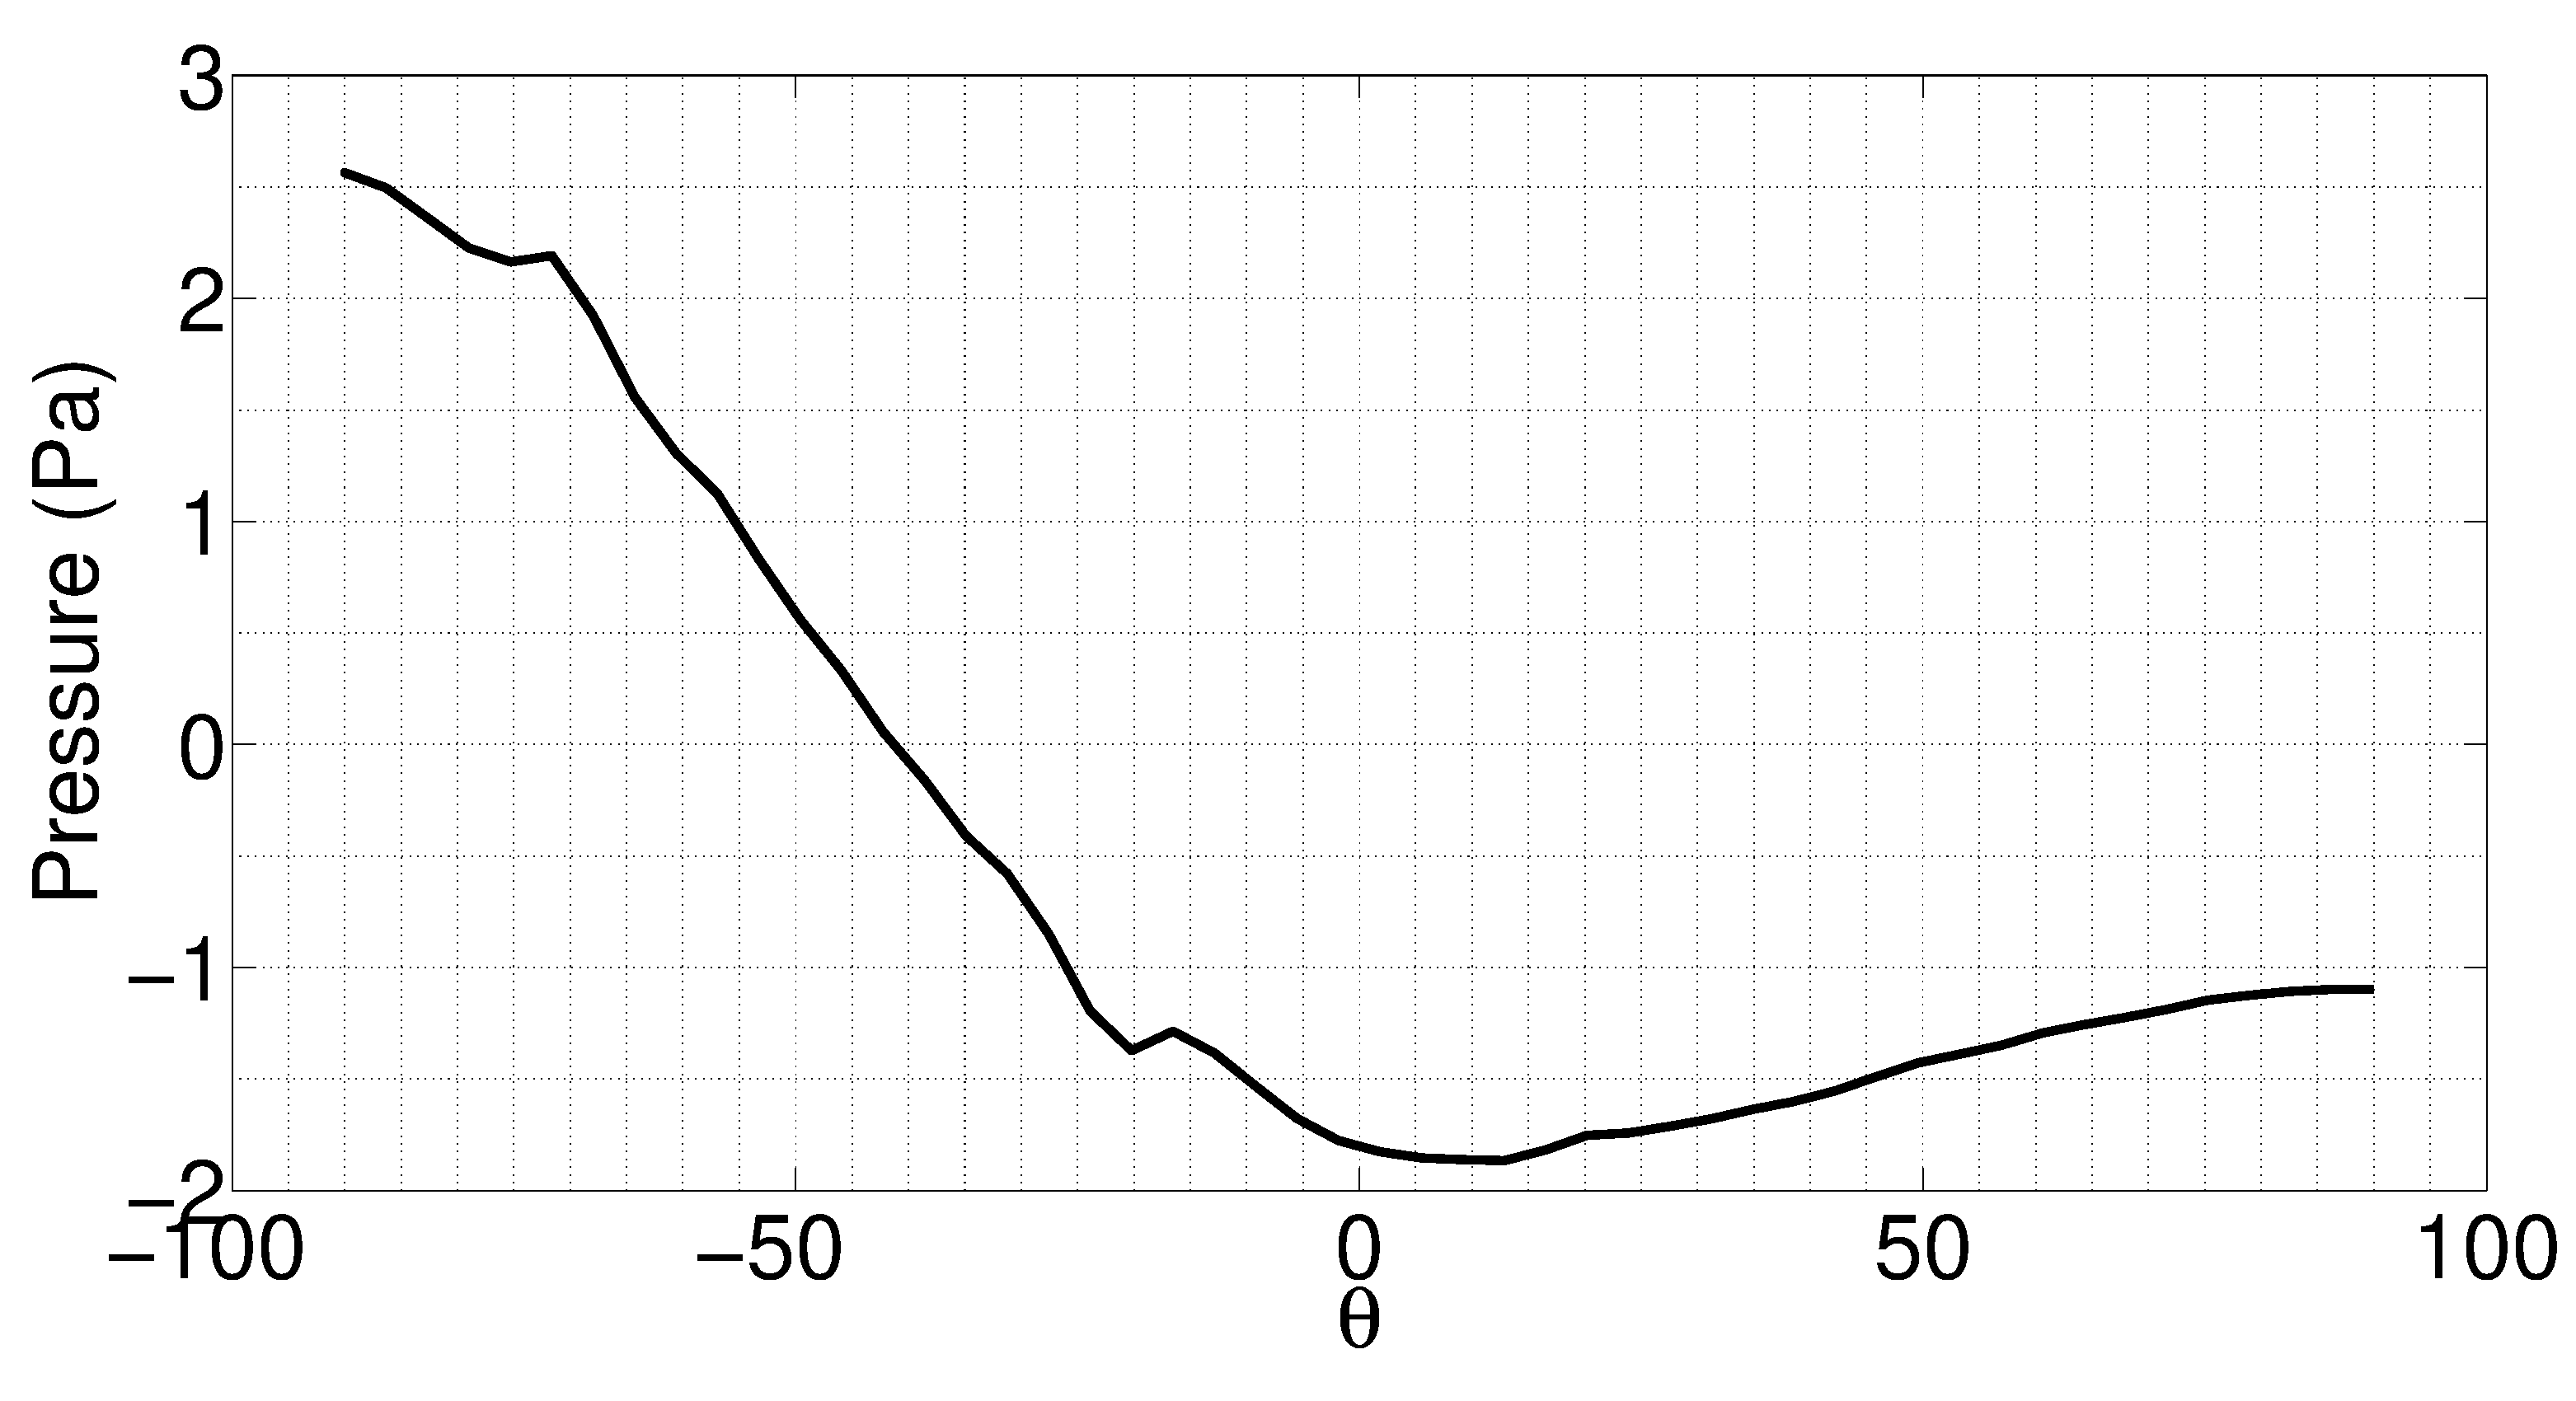
\includegraphics[width=12.00cm]{Chapter_4/figure/flow_over_cylinder/p_on_boundary_RE100.eps}
    \caption{Physical domain with dimensions for flow over cylinder.}
    \label{fig:C4_pressureOnSurfaceCylinder}
\end{figure}

The continuum sensitivity equation are derived by differentiating the governing NS equations of \eqref{eq:C4_NSwithvirtualBoundaryIB} with respect to the shape design variable, $b$, as shown in Equation \eqref{eq:C4_NSwithvirtualBoundaryIBsensitivity}. For this problem, the boundary on the cylinder is defined using the following analytical level-set function. For the points on the surface of the cylinder, Equation \eqref{eq:C4_levelSetFunctionForCylinder} is equal to zero.

\begin{equation}\label{eq:C4_levelSetFunctionForCylinder}
	\mathcal{R}(x, y; r): (x - x_0)^2 + (y - y_0)^2 = r^2
\end{equation}

For the sensitivity analysis, $\partial D/\partial X$ is calculated easily since the analytical form of the RD function is known (Equation \eqref{eq:C4_deltaFunction}). It is possible to calculate the $\partial X/\partial b$ values in Equation \eqref{eq:C4_NSwithvirtualBoundaryIBsensitivity} by differentiating Equation \eqref{eq:C4_levelSetFunctionForCylinder}. This is done in Equation \eqref{eq:C4_levelSetFunctionForCylinderSA}.

\begin{equation}\label{eq:C4_levelSetFunctionForCylinderSA}
	\frac{\partial \mathcal{R}(x, y; r)}{\partial b}: 
	2 (x - x_0)\dfrac{\partial x}{\partial b} + 
	2 (y - y_0)\frac{\partial y}{\partial b} = 
	2 r \frac{\partial r}{\partial b}
\end{equation}

For this analysis, the design variable $b$ is selected as the radius of the cylinder. Therefore, the right-hand-side of Equation \eqref{eq:C4_levelSetFunctionForCylinderSA} reduces to $2r$.

The boundary conditions for the sensitivity analysis are defined by differentiating the original boundary conditions of the governing equations. These conditions does not depend on the design variables and therefore, have zero values. Having the governing equations and boundary conditions, it is possible to solve the sensitivity equations.

The complex step method is used to validate the sensitivity response of the system. As mentioned in Chapter \ref{ch:introduction}, the complex step method does not have the accuracy issues of the finite different method and provides the accurate sensitivities upto machine precision. However, the analysis code requires to handle complex arithmetic. The analysis code is developed in MATLAB using the guidelines of \cite{martins2003complex} so that complex step can be used to calculating the sensitivities. The complex step derivative is defined in Equation \eqref{eq:C1_compelxStepFormula}.